
\ifdefined\ismainfile
\else
    \documentclass[11pt]{article}
    
    \makeatletter
\@ifclassloaded{revtex4-2}{}{\usepackage[margin=1in]{geometry}}
\makeatother
\usepackage{amsmath,amsthm,amsfonts,amssymb,mathrsfs}
\usepackage{graphicx}
\usepackage{cancel}
\usepackage{bm}
\usepackage{tikz}
\usepackage{csquotes}
\usepackage{tikz-3dplot}
\usepackage{physics}
\usepackage{dsfont}
\usepackage{float}
\usepackage{xcolor}
\usepackage{mathtools}
\usepackage{tcolorbox}
\makeatletter
\@ifclassloaded{revtex4-2}{\let\affil\affiliation
}{\usepackage{authblk}}
\makeatother

\tcbuselibrary{breakable}
\usepackage{keytheorems}
\newkeytheorem{definition}[parent=section, tcolorbox-no-titlebar={breakable, colback=blue!10}]
\newkeytheorem{example,lemma,conjecture,claim,theorem,proposition,corollary,fact,assumption,construction}[sibling=definition, tcolorbox-no-titlebar={breakable, colback=blue!10}]
\theoremstyle{definition}
\newtheorem{protocol}{Protocol}[section]

\newkeytheorem{remark}[parent=section, tcolorbox-no-titlebar={breakable}]
\allowdisplaybreaks[4]
\interdisplaylinepenalty=0
\makeatletter
\renewcommand{\log}{\mathop{\operator@font log}\nolimits}
\makeatother
\IfFileExists{bbm.sty}{\usepackage{bbm}}{\providecommand{\mathbbm}{\mathds}}
\usepackage{stmaryrd}
\usepackage{braket}
\makeatletter
\@ifpackageloaded{natbib}{}{\usepackage[numbers,sort&compress]{natbib}}
\makeatother
\usepackage{hyperref}
\usepackage[ruled,noline,longend]{algorithm2e}
\SetAlgoNoLine
\AtBeginDocument{\SetAlgoNoLine}
\SetAlgoLongEnd
\RestyleAlgo{boxruled}
\LinesNumbered
\definecolor{algcommentgray}{gray}{0.35}
\newcommand{\AlgCommentFont}[1]{\textcolor{algcommentgray}{#1}}
\SetCommentSty{AlgCommentFont}
\SetKwComment{tcp}{{\color{algcommentgray}$\blacktriangleright$}\ }{}
\usepackage{tcolorbox}
\tcbuselibrary{breakable}
\renewcommand{\topfraction}{0.9}
\renewcommand{\bottomfraction}{0.8}
\renewcommand{\textfraction}{0.07}
\renewcommand{\floatpagefraction}{0.85}
\setcounter{topnumber}{3}
\setcounter{totalnumber}{5}
\newenvironment{longalgorithm}[2][]{\begin{tcolorbox}[breakable, sharp corners, boxsep=0pt,
      boxrule=\algoheightrule, colframe=black, colback=white,
      left=18pt, right=4pt, top=5pt, bottom=5pt, #1]\refstepcounter{algocf}\noindent\hspace*{-14pt}{\textbf{\algorithmcfname~\thealgocf:} #2}\par
  \addcontentsline{loa}{algocf}{\protect\numberline{\thealgocf}#2}\par\nobreak\vspace{2pt}\nointerlineskip
  \moveleft18pt\vbox{\hrule width \dimexpr\linewidth+22pt\relax height \algoheightrule}\vspace{3pt}\setcounter{AlgoLine}{0}\RestyleAlgo{plain}}{\end{tcolorbox}}
\DontPrintSemicolon
\SetKwInput{KwIn}{Require}
\SetKwInput{KwOut}{Ensure}
\SetKwFor{For}{for}{do}{end for}
\SetKwFor{ForEach}{for each}{do}{end for}
\SetKwFor{While}{while}{do}{end while}
\makeatletter
\newenvironment{breakablealgorithm}{\par\addvspace{\intextsep}\hrule height .8pt\kern2pt
  \renewcommand{\caption}[2][]{\refstepcounter{algocf}\noindent\textbf{\algorithmcfname~\thealgocf:} ##2\par
    \kern2pt\hrule\kern2pt
    \ifx\relax##1\relax
      \addcontentsline{loa}{algocf}{\protect\numberline{\thealgocf}##2}\else
      \addcontentsline{loa}{algocf}{\protect\numberline{\thealgocf}##1}\fi
  }}{\par\kern2pt\hrule\addvspace{\intextsep}}
\makeatother
\usepackage{old-arrows}
\usepackage{color}
\usepackage{array, tabularx}
\usepackage{longtable}
\makeatletter
\@ifclassloaded{revtex4-2}{\appdef\@mkpream@relax{\let\@endpbox\relax}}{}
\makeatother
\usepackage{booktabs}
\newcolumntype{L}[1]{>{\raggedright\arraybackslash}p{#1}}
\newcolumntype{C}[1]{>{\centering\arraybackslash}p{#1}}
\newcolumntype{R}[1]{>{\raggedleft\arraybackslash}p{#1}}
\newcommand{\Circo}[0]{\mathfrak{C}}
\newcommand{\restrict}[2]{#1 \vert_{#2}}
\newcommand{\physq}[0]{\mathcal{M}}


\newcommand{\Xp}[0]{\mathcal{X}}
\newcommand{\Zp}[0]{\mathcal{Z}}

\newcommand{\nS}[1]{\mathbb{N}_{#1}}
\newcommand{\aS}[1]{\mathbb{C}_{#1}}

\newcommand{\nD}[1]{D^N_{#1}}
\newcommand{\aD}[1]{D^C_{#1}}

\newcommand{\control}[3]{C_{#1} {#2}_{#3}}
\usetikzlibrary{3d, shapes, arrows.meta, decorations.pathreplacing, decorations.markings, cd, shapes.geometric, calc}
\IfFileExists{tikzlibrarycalligraphy.code.tex}{\usetikzlibrary{calligraphy}}{}
\pgfkeysifdefined{/pgf/decoration/calligraphic brace/.@cmd}{}{\pgfkeys{/pgf/decoration/calligraphic brace/.style={brace}}}
\tikzstyle{midarrow} = [decoration={markings, mark= at position 0.6 with {\arrow{Stealth}}}, postaction={decorate}]
\renewcommand{\comment}[1]{{\color{red} #1}}

\newcommand{\YR}[1]{{\color{Teal} [Collin: #1]}}

\newcommand{\kc}[1]{{\color{cyan} [Katie: #1]}}

\newcommand{\bb}[1]{{\color{purple}[BB: #1]}}




\newcommand{\vva}[1]{{\color{magenta} [VVA: #1]}}









\newcommand{\al}[1]{{\color{DarkGreen} [Ana: #1]}}

\newcommand{\hp}[1]{{\color{brown} [Harry: #1]}}

\newcommand{\NT}[1]{{\color{orange} [NT: #1]}}

\newcommand{\dom}[1]{\textcolor{blue}{[Dom: #1]}}

\newcommand{\todo}[1]{\textcolor{blue}{[TO-DO: #1]}}

\newcommand{\new}[1]{{\color{DarkMagenta}#1}}
\definecolor{FGreen}{RGB}{58,158,92}
\definecolor{lightred}{RGB}{223, 123, 84}
\definecolor{lightbrown}{RGB}{242,216,199}
\definecolor{invisiblegray}{RGB}{238,238,237}
\definecolor{lightgreen}{RGB}{222, 235, 218}
\definecolor{lightcyan}{RGB}{153, 191, 216}
\definecolor{lightcyan2}{RGB}{208, 224, 235}
\definecolor{cyan2}{RGB}{144,201,226}
\definecolor{lightyellow}{RGB}{252, 238, 183}
\definecolor{OrangeRed}{RGB}{223,123,84}
\definecolor{CyanGreen}{RGB}{81,177,184}
\definecolor{rose}{RGB}{226,45,139}
\definecolor{Ycolor}{RGB}{248,236,104}
\definecolor{Hcolor}{RGB}{255,255,0}
\definecolor{Xcolor}{RGB}{246,143,138}
\definecolor{Zcolor}{RGB}{210,254,206}
\definecolor{Lred}{RGB}{244,163,163}
\definecolor{Lgreen}{RGB}{160,211,179}
\definecolor{Lblue}{RGB}{170,183,240}
\definecolor{tickcolor}{RGB}{181,0,250}
\definecolor{DarkBlue}{RGB}{14,38,80}
\definecolor{greenblue}{RGB}{0,255,127}
\definecolor{darkblue}{RGB}{57,85,134}
\definecolor{electrored}{RGB}{244,96,85}
\definecolor{electrored2}{RGB}{245,107,94}
\definecolor{BBXcheck}{RGB}{210,234,206}
\definecolor{BBZcheck}{RGB}{204,204,250}
\definecolor{softred}{RGB}{245,206,206}
\definecolor{fuchsiapurple}{RGB}{180, 0, 255}
\definecolor{Teal}{RGB}{62,138,141}
\definecolor{gold}{RGB}{233,168,58}
\definecolor{Crimson}{RGB}{220,20,60}
\definecolor{RedOrange}{RGB}{255,69,0}
\definecolor{DarkMagenta}{RGB}{139,0,139}
\definecolor{DarkGreen}{RGB}{0,100,0}
\definecolor{MidnightBlue}{RGB}{25,25,112}



\newcommand{\g}{\mathbf{g}}
\newcommand{\h}{\mathbf{h}}
\renewcommand{\k}{\mathbf{k}}
\newcommand{\f}{\mathbf{f}}
\newcommand{\C}{\mathbf{C}}
\newcommand{\Z}{\mathbb{Z}}
\renewcommand{\S}{\mathcal{S}}
\newcommand{\CC}{\mathcal{C}}
\newcommand{\charge}{k}
\newcommand{\totalcharge}{K}
\newcommand{\B}{\mathbb{B}}
\renewcommand{\O}{\mathcal{O}}
\newcommand{\Ocal}{\mathcal{O}}
\renewcommand{\Vec}{\mathcal{V}ec}
\newcommand{\Rep}{\text{Rep}}
\newcommand{\nnb}{\nonumber}
\newcommand{\lt}{\triangleleft}
\newcommand{\rt}{\triangleright}
\newcommand{\Lcal}{\mathcal{L}}
\newcommand{\Acal}{\mathcal{A}}
\newcommand{\Gcal}{\mathcal{G}}
\newcommand{\XX}{\mathcal{X}}
\newcommand{\YY}{\mathcal{Y}}
\newcommand{\ZZ}{\mathcal{Z}}
\newcommand{\Com}[2]{[ #1, #2 ]}
\newcommand{\ComGrp}[2]{[ #1, #2 ]_{\text{grp}}}
\newcommand{\level}{\operatorname{Lv}}
\newcommand{\code}{\mathcal{C}}


\newcommand{\glosym}[0]{\mathsf{L}}
\newcommand{\im}{\operatorname{im}}
\newcommand{\rk}{\operatorname{rk}}
\newcommand{\supp}[1]{\operatorname{Supp}(#1)}
\newcommand{\Ad}{\operatorname{Ad}}
\newcommand{\Irrep}{\operatorname{Irrep}}
\newcommand{\Wt}{\operatorname{Wt}}
\newcommand{\Lin}{\mathfrak{L}}
\newcommand{\interior}{\operatorname{int}}
\newcommand{\T}[0]{\mathsf{U}}
\newcommand{\orbit}[1]{O^{\mathcal{T}}(#1)}
\newcommand{\sym}[0]{\overline{S}}
\newcommand{\av}[0]{\mathbb{A}_v}
\newcommand{\bp}[0]{\mathbb{B}_f}
\newcommand{\onsite}[1]{\mathsf{T}|_{#1}}
\newcommand{\Log}[1]{\overline{#1}}
\newcommand{\id}[0]{\mathbf{1}}
\newcommand{\bd}[1]{\delta({#1})}
\newcommand{\zp}[0]{\mathbb{Z}_p}
\newcommand{\cX}[0]{\mathcal{X}}
\newcommand{\cZ}[0]{\mathcal{Z}}
\newcommand{\cC}[0]{\mathcal{C}}
\newcommand{\cE}[0]{\mathcal{E}}
\newcommand{\cx}[2]{CX_{#1\rightarrow#2}}
\newcommand{\wcp}[2]{\mathcal{C}P_{#1\rightarrow#2}}
\newcommand{\wcx}[2]{\mathcal{C}X_{#1\rightarrow#2}}
\newcommand{\wcz}[2]{\mathcal{C}Z_{#1\rightarrow#2}}
\newcommand{\wcy}[2]{\mathcal{C}Y_{#1\rightarrow#2}}
\newcommand{\cpw}[2]{C\mathcal{P}_{#1\rightarrow#2}}
\newcommand{\cxw}[2]{C\mathcal{X}_{#1\rightarrow#2}}
\newcommand{\czw}[2]{C\mathcal{Z}_{#1\rightarrow#2}}
\newcommand{\cyw}[2]{C\mathcal{Y}_{#1\rightarrow#2}}
\newcommand{\wct}[2]{\mathcal{C}\mathcal{T}_{#1\rightarrow#2}}
\newcommand{\wctdag}[2]{\mathcal{C}\mathcal{T}^\dagger_{#1\rightarrow#2}}
\newcommand{\cnot}[0]{\CNOT}
\newcommand{\SWAP}[0]{\mathsf{SWAP}}
\newcommand{\CNOT}[0]{\mathsf{CNOT}}
\newcommand{\CSWAP}[0]{\mathsf{CSWAP}}
\newcommand{\CX}[0]{\mathsf{CX}}
\newcommand{\CZ}[0]{\mathsf{CZ}}
\newcommand{\CT}[0]{\mathsf{CU}}
\newcommand{\swap}[0]{\SWAP}
\newcommand{\cswap}[0]{\CSWAP}

\newcommand{\overlap}[1]{\Omega(#1)}
\newcommand{\E}[2]{e_{(#1,#2)}}
\newcommand{\dec}[1]{\tilde{#1}}
\newcommand{\insuppof}[2]{#1|_{#2}}
\newcommand{\plushalf}[1]{{#1+\frac{1}{2}}}
\newcommand{\minushalf}[1]{{#1-\frac{1}{2}}}
\newcommand{\scrG}[0]{{\mathscr{G}}}
\newcommand{\sset}[1]{\Sigma(#1)}

\newcommand{\symOP}{\T}
\newcommand{\symS}{\overline{S}}
\newcommand{\haH}{\mathsf{H}}
\newcommand{\haA}{\mathsf{A}}
\newcommand{\haB}{\mathsf{B}}
\newcommand{\haP}{\mathsf{P}}
\newcommand{\haQ}{\mathsf{Q}}
\newcommand{\haX}{\mathsf{X}}
\newcommand{\Deco}{\mathfrak{D}}

\newcommand{\vertexset}[1]{\Sigma^{-1}(#1)}
\newcommand{\invvertexset}[1]{\Sigma(#1)}
\newcommand{\faceP}{\mathcal{P}} 
\newcommand{\vertexV}{\mathsf{V}}
\newcommand{\edgeE}{\mathsf{E}}
\newcommand{\faceF}{\mathsf{F}}
\newcommand{\graphG}{\mathsf{G}}
\newcommand{\intG}{\mathbb{G}}
\newcommand{\N}{\mathsf{N}}
\newcommand{\eigenE}{\mathbf{E}} 
\newcommand{\gaugedA}{\mathbb{A}}
\newcommand{\gaugedB}{\mathbb{B}}
\newcommand{\gaugedS}{\mathbb{S}}
\newcommand{\Sdec}{\mathfrak{s}}
\providecommand{\vr}{}
\renewcommand{\vr}{v_r}
\newcommand{\gaugedH}{\mathbb{H}}
\newcommand{\gaugingOP}{\mathscr{G}}
\newcommand{\chproj}[2]{\llbracket #1\rrbracket _{#2}}

\newcommand{\gX}{\mathcal{X}}
\newcommand{\gZ}{\mathcal{Z}}
\newcommand{\mX}{\mathcal{X}}
\newcommand{\mZ}{\mathcal{Z}}
\newcommand{\gW}{\mathcal{W}}
\newcommand{\gY}{\mathcal{Y}}
\newcommand{\Agrp}{\mathbf{A}}
\newcommand{\chOmega}{\mathit{\Omega}}
\newcommand{\Linex}{\Lin_{\rm ex}(\mathcal H_{\rm m})}
\newcommand{\Linnt}{\Lin_{\rm nt}^{\rm ex}(\mathcal H_{\rm mat})}


\newcommand{\K}{\mathcal{K}}
\newcommand{\gaugedT}{\mathbb{T}}
\newcommand{\Stab}{\mathcal{G}}
\newcommand{\F}{\mathcal{F}}
\newcommand{\Hp}{\mathcal{H}}
\newcommand{\Poly}{\mathsf{Poly}}
\newcommand{\Fphys}{F_{\text{phys}}}
\newcommand{\Fmeas}{F_{\text{meas}}}
\newcommand{\Fp}{\mathbf{F}_p}
\newcommand{\Zq}{\mathbb{Z}_q}
\newcommand{\Sprod}[2]{\Lambda\left( #1, #2 \right)}
\newcommand{\FT}{F^T}
\newcommand{\nbhd}{\mathsf{N}}

\newcommand{\Cgeom}{C_{\text{geom}}}
\newcommand{\CLDPC}{C_{\text{LDPC}}}
\newcommand{\Cstep}{C_{\text{step}}}
\newcommand{\Cretract}{C_{\text{retract}}}
\newcommand{\Ctotal}{C_{\text{total}}}
\newcommand{\Cgauge}{C_{\text{gauge}}}

\newcommand{\nonabel}[1]{S^\mathrm{N}_{#1}}
\newcommand{\abel}[1]{S^\mathrm{A}_{#1}}
\newcommand{\gnonabel}[1]{\mathbb{S}^\mathrm{N}_{#1}}
\newcommand{\gabel}[1]{\mathbb{S}^\mathrm{A}_{#1}}
\newcommand{\onset}[2]{{#1}_{\sset{#2}}}
\newcommand{\ccomm}[2]{[#1,#2]_{\mathrm{grp}}}
\newcommand{\tu}[0]{t_{\mathrm{u}}}
\newcommand{\tg}[0]{t_{\mathrm{g}}}
\newcommand{\tf}[0]{t_\mathrm{f}}
\newcommand{\Ig}[0]{\mathrm{I}_{\mathrm{g}}}
\newcommand{\Ifn}[0]{\mathrm{I}_\mathrm{f}}
\newcommand{\Ib}[0]{\mathrm{I}_0}
\newcommand{\cA}[0]{\mathcal{A}}
\newcommand{\cQ}[0]{\mathcal{Q}}
\newcommand{\cK}[0]{\mathcal{K}}
\newcommand{\grpcom}[2]{\ComGrp{#1}{#2}}
\newcommand{\de}[0]{d_\mathcal{E}}



\definecolor{Teal}{RGB}{0,128,128}
\definecolor{Crimson}{RGB}{220,20,60}
\definecolor{RedOrange}{RGB}{255,69,0}
\definecolor{DarkMagenta}{RGB}{139,0,139}
\definecolor{DarkGreen}{RGB}{0,100,0}
\definecolor{MidnightBlue}{RGB}{25,25,112}


\hypersetup{
    colorlinks=true,
    linkcolor=MidnightBlue,
    citecolor=MidnightBlue,
    urlcolor=MidnightBlue,}

\usepackage{amsfonts,latexsym,amsthm,amssymb,amsmath,amscd,euscript,tikz,mathtools}
\usepackage{framed}
\usepackage[normalem]{ulem}
\makeatletter
\@ifclassloaded{revtex4-2}{}{\usepackage[margin=1in]{geometry}}
\makeatother
\usepackage{color}




\usepackage{enumitem}
\usepackage{environ}
\usepackage{dcolumn}

\usetikzlibrary{positioning, shadows, arrows, backgrounds, fit}
\usetikzlibrary{decorations.pathmorphing}

\definecolor{Teal}{RGB}{0,128,128}

\hypersetup{
    colorlinks=true,
    linkcolor=MidnightBlue,
    citecolor=MidnightBlue,
    urlcolor=MidnightBlue,
}

\definecolor{GrayOut}{gray}{0.8}
\NewEnviron{GrayedOut}{\begingroup\color{GrayOut}\BODY\endgroup
}

\newcommand{\diam}{\operatorname{diam}}
\newcommand{\dist}{\operatorname{dist}}

\newcommand{\cH}{\mathcal{H}}
\newcommand{\cT}{\mathcal{T}}
\newcommand{\cN}{\mathcal{N}}
\newcommand{\cB}{\mathcal{B}}
\newcommand{\bbP}{\mathbb{P}}
\newcommand{\haT}{\mathsf{T}}
\newcommand{\haD}{\mathsf{D}}
\newcommand{\cF}{\mathcal{F}}

\newcommand{\CZero}{C_0(\Gcal_0)}
\newcommand{\COne}{C_1(\Gcal_1)}
\newcommand{\deltaOne}{\delta_1}
\newcommand{\jall}{\mathbf{1}}
\newcommand{\tof}[0]{\ket{\mathsf{Tof}}}
\newcommand{\Pp}[1]{\mathrm{P}^+_{\Log{#1}}}
\newcommand{\Ppk}[1]{\mathrm{P}^+_{\Log{#1}^{\otimes k}}}
\newcommand{\Pm}[1]{\mathrm{P}^-_{\Log{#1}}}

\newcommand{\fa}[0]{F_\mathrm{A}}
\newcommand{\fn}[0]{F_\mathrm{N}}

\newcommand{\CHANGE}[1]{{\color{DarkMagenta}#1}}

\newcommand{\syndromeSet}{\sigma}
\newtheorem{axiom}{Axiom}[section]
\newtheorem{question}{Question}[section]


\newcommand{\green}[1]{\textcolor{Teal}{#1}}
\newcommand{\blue}[1]{\textcolor{blue}{#1}}
\newcommand{\red}[1]{\textcolor{red}{#1}}

\makeatletter
\let\UncappedLeft\left
\let\UncappedRight\right
\def\left{\@ifnextchar({\CappedLeftParen}{\UncappedLeft}}
\def\CappedLeftParen(#1\right{\@ifnextchar){\CappedRightParen{#1}}{\UncappedLeft(#1\UncappedRight}}
\def\CappedRightParen#1){\mathopen{}\bigg(#1\bigg)\mathclose{}}
\makeatother

\definecolor{vred}{rgb}{0.85,0,0}
\definecolor{epur}{cmyk}{0.45,0.86,0,0}
\definecolor{poraBase}{cmyk}{0,0.42,1,0}
\colorlet{pora}{poraBase!90!black}
\definecolor{setgray}{RGB}{225,225,225}
\newcommand{\vC}[1]{{\color{vred}#1}}
\newcommand{\eC}[1]{{\color{epur}#1}}
\newcommand{\pC}[1]{{\color{pora}#1}}
\newcommand{\sq}[9]{\left(\begin{smallmatrix}
\vC{#1} & \eC{#2} & \vC{#3}\\[1pt]
\eC{#4} & #5 & \eC{#6}\\[1pt]
\vC{#7} & \eC{#8} & \vC{#9}
\end{smallmatrix}\right)}
\newcommand{\mm}[4]{\begin{smallmatrix}#1 & #2\\ #3 & #4\end{smallmatrix}}
\newcommand{\sqe}[5]{\sq{\cdot}{#1}{\cdot}{#2}{#3}{#4}{\cdot}{#5}{\cdot}}
\newcommand{\Sg}{\mathsf{S}}
\newcommand{\CZbar}{\overline{CZ}}

\setcounter{tocdepth}{1}

    
    \author{}
    \title{Fault tolerance of the gauging procedure}
    
    \begin{document}
    
    
    \maketitle

\fi

In this section, we establish our main result: a lower-bound on the spacetime fault distance of the gauging procedure (Def.~\ref{def:detailed-gauging-procedure}).
Two features distinguish this setting from the fault-distance analysis in Pauli codes, requiring new machinery. 
First, the measured checks of the gauged code $\cC'$ are unitary but in general neither Hermitian nor Pauli, so a data fault need not commute or anti-commute with a check. Such faults are labeled ``non-Abelian'', and they act to randomize certain detectors. 
Second, a pair of decorated checks commute only up to a Pauli element of the check group (Theorem~\ref{cor:z2-commutation-relations}) and so outside of the codespace, the measurement of one check
can randomize another. 
Both of these mechanisms create would-be detectors whose values are 
random rather than deterministic, which we refer to as \emph{dropped detectors} 
(Definition~\ref{def:detectors}).

Here, we focus on lower bounding the weight of an undetectable fault configuration, where undetectable means that no deterministic detectors are violated. Such fault configurations are called \emph{loop-like} (Def. ~\ref{def:loop-like-fault}).
We prove that dropped detectors are localized to a constant-sized bounded region around any loop-like fault (Lemma ~\ref{lem:dropped-detector-localization}).
Further, we introduce a new variant of the standard cleaning argument (Section~\ref{sec:cleaning}) that deals with multiple measurement trajectories consistent with the same fault pattern. Using this cleaning argument, we map any loop-like fault on the gauging protocol, that is below a certain weight, onto a logically trivial operator on the ungauged code (Thm. \ref{thm:spacetime-distance}). We provide an informal statement of the main theorem and a proof sketch below.
\vspace{3pt}


\begingroup
\setlength{\LTleft}{0pt plus 1fill}
\setlength{\LTright}{0pt plus 1fill}
\begin{longtable}{@{}p{0.30\linewidth}p{0.67\linewidth}@{}}
    \hline
        Notation & Denotes \\
    \hline
    \endfirsthead
    \hline
        Notation & Denotes \\
    \hline
    \endhead
    \endfoot
    \caption{Notation used for this section.}
    \label{tab:sec-4-notation}
    \endlastfoot
        d & distance of $\cC$\\
        $O(\cdot)$ & Landau notation with respect to a family of codes with $d\to\infty$.\\
        $d_f$ & Fault distance of the gauging protocol. \\
        $\mathbb{C} \in \cA,\mathbb{N} \in \cN$ & Measured Abelian and non-Abelian checks of $\cC'$. $\cA$-checks detect Abelian faults. $\cN$-checks detect non-Abelian faults.\\
        $f, f_N, f_A$ & Elementary faults, non-Abelian elementary faults, Abelian elementary fault.\\
        $F, F_N, F_A$ & Fault configuration, non-Abelian component, Abelian component. \\
        $\lambda(Q)$ & Spectrum of operator $Q$. \\
        $(Q,t)$ & Measurement event of operator $Q$ at time $t$.\\
        $r(Q, t)$ & Measurement outcomes for a particular quantum trajectory in the absence of noise.\\
        $r_F(Q, t)$ & Noisy measurement outcomes in the presence of a fault configuration $F$. \\
        $E_F(t)$ & Support of fault $F$ on timestep $t$. \\
        $M_t(r, r_F)$ & Projective measurements performed at timestep $t$ to recreate measurement trajectory $r(Q, t)$. \\
        $K(F, r)$, $K(\emptyset, r)$ & Kraus operator corresponding to trajectory $(F, r)$. When $F = \emptyset$, it indicates a fault-free trajectory. \\
        $m_\T(r_F)$ & Inferred value of the operator $\T$ from faulty measurement trajectory $r_F$. \\
        $D_Q^t(r_F)$ & Detector value for operator $Q$ at time $t$, given faulty trajectory $r_F$. \\
        $\cA$-detector, $\cN$-detector & detectors made of measurement outcomes of $\cA$-checks and $\cN$-checks, respectively.\\
        $\text{Drop}(F)$ & Set of detectors randomized by the presence of some fault. Always $\cA$-detectors. \\
        $\mathcal{H} = (V_\mathcal{H}, E_\mathcal{H})$ & Fault location hypergraph. Vertices are fault locations, hyperedges are detectors whose outcome is impacted by its boundary faults. \\
        $\mathsf{N}_\xi (D)$ & Neighborhood around detector $D$ on the fault location hypergraph $\mathcal{H}$ of radius $\xi$. \\
        $\mathrm{Err}(R)$ & All linear combinations of all products of faults generated by some set of elementary spatial faults $R$. \\
        $\cB_t$ & The set of all Abelian byproducts that arise when we move non-Abelian faults supported at time $t$ forward or backward in time. \\
        
\end{longtable}
\endgroup


\subsection{Proof sketch}

We restrict to an order-two transversal symmetry $\T$, so that $\T^2 = \id$. As a result, this restricts to the case of gauge \textit{qubits} instead of qudits of dimension $p$, but for consistency, we still use $\cX,\cZ$ to denote Paulis on gauge qubits.
Let $\cC$ be the base code with distance $d$ and let $\cC'$ be its gauged code with gauging graph $\graphG =(\vertexV,\edgeE)$ that satisfies the desiderata in Def.~\ref{def:graph-desiderata}.

From the stabilizers defined in Thm.~\ref{thm:z2-gauged-stabilizers} and Cor.~\ref{cor:z2-commutation-relations}, take $\{\aS{i}\}_i = \{\av\} \sqcup (\{\gaugedS\}/\{\mathbb{N}_S\})$.
Throughout this section, we consider measuring the following stabilizer generators of $\cC'$,
\begin{align}
\label{eq:measured-checks}
    \cA := \{\aS{i}\}_{i},\qquad \cN:=\{\nS{j}\}_j = \{\bp\} \sqcup \{\mathbb{N}_S\} \cup \{\grpcom{\aS{i}}{\aS{k}}:i<k,\  \grpcom{\aS{i}}{\aS{k}} \neq \id
    )\} .
\end{align}
We refer to stabilizers in $\cA$ and $\cN$ as Abelian and non-Abelian stabilizers, respectively (see Table~\ref{tab:checks}).
Using Cor.~\ref{cor:z2-commutation-relations}, $\grpcom{\aS{i}}{\aS{k}}\in \langle \{\nS{j}\}_j \rangle$, so stabilizers in $\{\grpcom{\aS{i}}{\aS{k}}:i<k,\  \grpcom{\aS{i}}{\aS{k}} \neq \id)\} $ are redundant and do not change $\cC'$. 
Furthermore, they are LDPC since $\supp{\grpcom{\aS{i}}{\aS{k}}}\subseteq \supp{\aS{i}}\cup \supp{\aS{k}}$. 
It can be verified using Cor.~\ref{cor:z2-commutation-relations} that, on the full Hilbert space, the measured checks in Eq.~\eqref{eq:measured-checks} satisfy
\begin{align}
    \grpcom{\nS{j}}{\nS{l}}=\grpcom{\nS{j}}{\aS{i}}=\id,\qquad \grpcom{\aS{i}}{\aS{k}}\in \langle \cN \rangle.
\end{align}
\noindent


\begin{theorem}[Spacetime fault distance, informal] 
Consider any possible execution of the gauging procedure containing fewer than $d/\gamma$ elementary faults.

If every detector that is not dropped has value $1$, then the execution agrees with some fault-free execution both on the protected logical information and measured outcome of $\T$.

Therefore, the gauging procedure in Def.~\ref{def:detailed-gauging-procedure} admits a constant $\gamma = O(1)$ such that the adversarial spacetime fault distance satisfies 
\[
d_\mathrm{f} \geq d/\gamma.
\]

\end{theorem}


\textbf{Proof sketch.} 
It suffices to consider fault configurations $F$ that violate no deterministic detectors. 
$\cN$-detectors, comprising the product of $\cN$ stabilizer outcomes, remain deterministic regardless of $F$.
We show every non-deterministic or dropped $\cA$-detector lies near a non-Abelian fault, and therefore the number of dropped detectors is $O(\Wt(F))$.
For any fault configuration $F$ with $\Wt(F)\le d/\gamma$ that violates no deterministic detector, we show there must exist a clean `cut' or connected set of qubits and measurement outcomes that are perfect in each of the pre-gauging, gauged, and post-gauging spacetime regions. This ensures that no logical readout error of the Clifford measurement has occurred. 

Cleaning faults away from these cuts rewrites the effect of $F$ as a linear combination of
errors at four rounds: the first round of $\cC$, the last round of $\cC$ before gauging, the first round of $\cC$ after gauging, and the last round of $\cC$. 
All terms in this linear combination are supported on common sets $(R_0,R_1,R_2,R_f)$ satisfying
\begin{equation}\label{eq:cleaning-common-support}
|R_0|+|R_1|+|R_2|+|R_f|=O(\Wt(F)).
\end{equation}
For a suitable constant $\gamma$, $O(\Wt(F))$ is smaller than the code distance of $\cC$. As these now purely spatial errors are sandwiched between clean codespace projectors, they must be correctable. 

The error spaces at these four rounds are therefore correctable, so no non-trivial logical action can occur on the codespace. Combined with the fact that no logical measurement error occurred, we conclude the fault we started with was trivial. Thus, any nontrivial fault must be larger than $d/\gamma$.

\subsection{Spacetime gauging procedure, faults, and trajectories} \label{sec:spacetime-setup}

\begin{table}
    \centering
    \begin{tabular}{|c|c|c|}
        \hline
         & \textbf{Detects} & \textbf{Commutation} \\
        \hline
        Abelian check $\in \cA$ & Abelian faults & Grp commutator $\in \cN$ (commutes in codespace)  \\
        Non-abelian check $\in \cN$ & Non-Abelian faults & Commuting \\
        \hline
    \end{tabular}
    \caption{Distinctions between Abelian checks $\cA$ and non-Abelian checks $\cN$. Abelian checks are called Abelian as they detect Abelian faults, although they do not commute with one another. Non-abelian checks commute, but they detect non-Abelian faults.}
    \label{tab:checks}
\end{table}

We now introduce the notation to define a measurement schedule for Abelian stabilizers that do not commute over the full Hilbert space. Define the non-commutation graph $\Gamma_\cA = (V_\cA, E_\cA)$ as 
\[
    V_\cA = \cA,\qquad E_\cA :=\{(\aS{i},\aS{k}): \grpcom{\aS{i}}{\aS{k}} \neq \id
    )\}.
\]
Fix a vertex-coloring of this graph, 
\[
\cA = \bigsqcup_{r=1}^\kappa \cA_r.
\]
A valid coloring is guaranteed to exist with $\kappa=O(1)$ colors because $\Gamma_\cA$ has $O(1)$-bounded degree; each generator $\aS{i}$ can only fail to commute over the full Hilbert space with a constant number of other stabilizers, because $\cC'$ is LDPC.



\begin{definition}[Fault-tolerant gauging procedure. Extended from Def.~\ref{def:gauging-measurement-protocol}]\label{def:detailed-gauging-procedure}
Let $\{S_i\}$ be the measured stabilizer generators of $\cC$.
Let $t$ be an integral time indexing the measurement round. 
The fault-tolerant gauging protocol is:
\begin{enumerate}
    \item For each $t=1,\dots,d$, measure all $S_i$ simultaneously.
    \item\label{step:gauging} After $t=d$ initialize $\ket{0}_e$ for each $e\in \edgeE$, and measure all $\av$ stabilizers simultaneously, following steps $1-2$ of Def.~\ref{def:gauging-measurement-protocol}.
    \item For each $t=d+1,\dots, 2d$, measure the $\cC'$ checks in subrounds $r=0,\dots ,\kappa$. In subround $r=0$, measure all checks in $\cN$ simultaneously. For subrounds $r=1,\dots,\kappa$, measure checks in $\cA_r$. (At round $t=d+1$, omit the $\av$ measurements that were already made in Step~2.)
    \item \label{step:ungauging} After $t=2d$, measure every $\cZ_e,\ e\in \edgeE$. 
    Then perform the feedforward local Clifford operation $U_{c(z)}$ (defined in Eq.~\eqref{eq:feedforward-clifford}).
    \item For each $t=2d+1,\dots,3d$,  measure each $S_i$.
\end{enumerate}
The protocol reports as its $\T$ outcome the product of all $\av$ measurement outcomes at $t=2d$.
\end{definition}

For completeness, we explicitly describe the Clifford feedforward operation in the presence of errors--- see Sec. \ref{sec:ungauging} for a discussion of the ideal, fault-free case. 

In step \ref{step:ungauging} of the gauging protocol, we measure out all of the edge ancilla in the $\Zp$ basis. Let $z\in \mathbb{F}_2^{|\edgeE|}$ be the recorded edge measurement string.

In the absence of faults, we have $\bp = +1$, which constrains the post-measurement state of the edge ancilla to look like $$\ket{z} = \prod_{v \in \Omega} \T_v \av \ket{0}$$ 
for some subset of vertices $\Omega \subseteq \vertexV$. 
In other words, the binary string $z$ must be a coboundary of the gauging graph: $\delta_2 z = 0$, where $z = \delta_1 \Omega$.
If some readout errors flipped the outcomes of the measurement, or there were some $\bp$ violations present prior to the measurement, we find $\delta_2 z \neq 0$. 

In the case of measurement errors, the true measurement outcome string $z^*$ is a coboundary, and we must simply determine the minimum weight correction that converts our faulty string $z$ into a coboundary.

Fix an ordering $e_1,\dots,e_{|\edgeE|}$ of the edges, and let $\prec$ denote this ordering on $\mathbb{F}_2^{|E|}$. 
Define
    \[
    \hat{e}(z) = \min_{\prec}\bigl(\rm{argmin}_{e\in \mathbb{F}_2^{|\edgeE|}}\bigl\{|e|:\delta_2(z+e)=0\bigr\}\bigr).
    \]
The purpose of the edge ordering is to ensure that $\hat{e}()$ is a deterministic function of $z$ when there are multiple minimum weight corrections.
Now fix a reference vertex $v_0$. Since $H^1(\graphG)=0$ and $\graphG$ is connected, there is a unique vector $c(z) \in \mathbb{F}_2^{|\vertexV|}$ satisfying
\[
    \delta_1 c(z)  = z+ \hat{e}(z),\qquad c(z)_{v_0} = 0.
\]
The Clifford feedforward correction applies the following operator on the matter qubits,
\begin{equation}
\label{eq:feedforward-clifford}
    U_{c(z)} :=\prod_{v:c(z)_v=1}\T_v.
\end{equation} which is simply the matter support of the product of $\av$ corresponding to the edge qubit coboundary.

In the second case where we also have some $\bp = -1$ violations, these violations are converted into deformations of the ungauged code~\cite{lyons2026}. Essentially, the state of the system after the ungauging measurement may have some amplitude outside of the $+1$ eigenspace for certain Pauli stabilizers of the base code. Thus, when we perform the first round of stabilizer measurements after measuring out the edge ancillas, we may observe some stabilizer violations. However, since we spend $d$ rounds in the ungauged code after step \ref{step:gauging}, there is ample time to identify such errors and correct them. We still want to perform the minimum-weight correction and Clifford feedback described above, however, to ensure that the weight of errors produced on the ungauged code remains bounded. 


\begin{definition}[Elementary faults]
\label{def:elementary-faults}
An \emph{elementary spatial fault} at time $t\in \{1,\dots, 3d\}$ is a nonidentity Pauli $f$, inserted immediately before round $t$, whose support lies entirely within one vertex set $\vertexset{v}$ or on one gauge qubit. We denote such spatial faults by $(t,f)$.

An \emph{elementary temporal fault} is a tuple $(t, Q, \pi)$, where an operator 
\[
Q\in \{S_i\}_i\cup \cN \cup \cA \cup \{\cZ_e\}_{e\in \edgeE}
\]
is measured at round $t$ in Def.~\ref{def:detailed-gauging-procedure}. Let $\lambda(Q)$ be the spectrum of eigenvalues of $Q$.
A temporal fault causes a permutation on measurement outcomes:
\[
\pi:\lambda(Q)\longrightarrow\lambda(Q).
\] 
In particular, if the projected eigenspace corresponds with the eigenvalue $r\in \lambda(Q)$, the recorded outcome is $\pi(r)$.
\end{definition}

\begin{definition}[Fault configuration]
    Let $\Lambda$ be the set of elementary faults allowed by Def.~\ref{def:detailed-gauging-procedure}.
    A \emph{fault configuration} is a finite set $F\subseteq \Lambda$ containing at most one temporal fault for each measurement. Its weight is $\Wt(F) := |F|$.
\end{definition}

\begin{definition}[Abelian and non-Abelian faults]
\label{def:abelian-non-abelian-faults}
    Consider a spatial fault $(t,f)$ where $t=[d+1,2d]$ (after Step~\ref{step:gauging} and before Step~\ref{step:ungauging} in Def.~\ref{def:detailed-gauging-procedure}). 
    This fault $f = f_A$ is \emph{Abelian} if 
    \begin{align}
        f_A\nS{j}=\nS{j}f_A,\qquad \nS{j}\in \cN.\label{eq:Fa-commutes-nS}
    \end{align}
    and 
    \begin{align}
        f^\dagger_A \aS{i} f_A \aS{i}^\dagger \in \{\pm \id \},\qquad\ \aS{i}\in \cA.
        \label{eq:abelian-condition-2}
    \end{align}
    A spatial fault is \emph{non-Abelian} otherwise, and denoted $f_N$.
    
    A temporal fault $(t, Q, \pi)$ is \emph{non-Abelian} when $Q\in \cN$ and \emph{Abelian} if $Q\in \cA$.
\end{definition}

\begin{remark}[Elementary faults on the ungauged code]
    Although there is no distinction between Abelian and non-Abelian faults on the base stabilizer code, it is convenient to consider the same elementary fault basis (in particular, the basis elements acting on the matter qubits) as we have defined above. Hence, we also label the faults as ``Abelian'' and ``non-Abelian'' on the base code. 
\end{remark}

Therefore, an Abelian spatial fault commutes with every $\nS{j}\in\cN$ and commutes or anticommutes with every $\aS{i}\in \cA$.
Consequently, it maps each $\aS{i}$-eigenspace to another eigenspace deterministically as opposed to a linear combination of eigenspaces, as with a regular Pauli fault.

Since every spatial fault $f$ and every $\nS{j}\in \cN$ are Pauli (recall the decorations to $\cN$ are simply $\Zp$ operators on the gauge edges), a non-Abelian spatial fault also maps each $\nS{j}$-eigenspace to another eigenspace deterministically. In contrast, it has unspecified action on the eigenspaces of checks in $\cA$.

During rounds in the base code $\cC$ ($t\notin [d+1,2d]$), we do not classify spatial or temporal faults as Abelian or non-Abelian. 
Let $\fn\subseteq F$ and $\fa\subseteq F$ denote non-Abelian and Abelian faults in $F$, respectively.

The next lemma shows that commuting an elementary non-Abelian spatial fault through a check in $\cA$ produces only a constant number of elementary Abelian spatial faults.
This is used below to bound the fault growth during the cleaning procedure.
\begin{lemma}[Non-Abelian faults leave behind a constant number of Abelian faults]
\label{lem:byproducts}
    There is a constant $\beta = O(1)$ such that, for every elementary non-Abelian spatial fault $(t, f_N)$ where $t\in \{d+1,\dots, 2d\}$ and every $\aS{i}\in \cA$, 
    \[
    f^\dagger_N \aS{i} f_N \aS{i}^\dagger = f_{A,1} f_{A,2} \cdots f_{A,m},\qquad m\le \beta
    \]
    up to a phase, where every nonidentity $f_{A,j}$ is supported within one vertex set or on one gauge qubit, $(t,f_{A,j})$ is Abelian, and 
    \[
    \supp{f_{A,j}}\subseteq \supp{\aS{i}}.
    \] 
\end{lemma}
\begin{proof}
    For a Pauli $P$ on $\vertexset{v}$, let us define its orbit product by 
    \[
    o(P) := P^\dagger \T_v P \T_v^\dagger.
    \]
    We refer to any Pauli operator that can be written as the above form as an \emph{orbit product}. We now show that $o(P)$ is an Abelian fault.
    Since $\T_v$ is Clifford, $o(P)$ is a Pauli on $\vertexset{v}$, and $\T_v^2 = \id$ gives $\T_v o(P) \T_v^\dagger = \pm o(P)$. 
    Suppose $\T_v M \T_v ^\dagger=\pm M$, and $PM = \epsilon MP$ for $\epsilon\in\{\pm 1\}$.
    Conjugating the latter relation by $\T_v$ gives 
    \[
    (\T_v P \T_v^\dagger) M = \epsilon M (\T_v P \T_v ^\dagger ).
    \]
    The two $\epsilon$ commutation signs cancel for $o(P) = (\T_v P \T_v^\dagger) \cdot P$, so 
    \[
    o(P)M = M o(P).
    \]

    First we show that $o(P)$ commutes with all checks in $\cN$.
    Let $M$ be the restriction to $\vertexset{v}$ of a stabilizer $N \in \cC$, where $N\T N \T = \id$. Since $N$ is invariant under $\T$, $N$ must satisfy $\T_v N \T_v^\dagger = \pm M$.
    Using our calculation above gives $[o(P),M]=0$, and therefore $[o(P),N]=0$. 
    Moreover, $o(P)$ acts only on matter qubits, so we must have $[o(P), \mathbb{N}] = 0$ as well. Similarly, $o(P)$ is disjoint from every $\bp$ check, and so commutes trivially. The remaining checks in $\cN$ are just products of gauged invariant checks $\mathbb{N}$ and $\bp$, so $[o(P),\nS{j}]$ for all $\nS{j}\in \cN$. 

    To verify the second Abelian condition in Eq.~\eqref{eq:abelian-condition-2}, recall the two forms of checks in $\cA$. 
    The vertex check is 
    \[\av = \T_v\prod_{e\in \delta(v)}\cX_e.
    \]
    If $u\neq v$, then $o(P)$ is disjoint from $\av$, so they commute. If $u=v$, then $\T_vo(P) \T_v^\dagger = \pm o(P)$ means $o(P)\av = \pm \av o(P)$.
    For a decorated check $\gaugedS$ associated with $S$ and with root vertex $v_0$, Thm~\ref{thm:z2-gauged-stabilizers} gives
    \[
    \gaugedS = S 
    \prod_{\substack{v\in \lambda (S)\\v\ne v_0}}
    \left(
    \mathsf{S}_{p(v,v_0)}^{\mu_v}
    \prod_{e\in p(v,v_0)}
    \mathrm{C_e}\bigl({N_{S}}_v\bigr)
    \right).
    \]
    Here, the $\mathsf{S}_{p(v,v_0)}^{\mu_v}$ acts only on the gauge qubits in $p(v,v_0)$ and is diagonal in the $\cZ$ basis, while 
    $\mathrm{C_e}\bigl( {N_{S}}_v\bigr)$ has edge control $e$ and matter target ${N_{S}}_v$. Moreover
    \[
    i^{\mu_v}(N_{S})_v = \grpcom{S_{v}}{\T_v},
    \]
    so each $(N_{S})_v$ is an orbit product up to a phase.

    Our earlier calculation shows that $o(P)$ commutes with every $({N_S})_u$, and therefore with every control gate $\mathrm{C}_e({N_S})_u$. Moreover, $o(P)$ is disjoint from $\mathsf{S}_{p(v,v_0)}^{\mu_v}$ so they commute, and since $S \in \cC$ is Pauli, the commutator with $S$ is a phase. Therefore, $o(P)\gaugedS = \pm \gaugedS o(P)$, and thus 
    \[
    o(P)^\dagger \aS{i} o(P) \aS{i}^\dagger\in \{\pm \id\},\qquad \aS{i}\in \cA,
    \]
    so each $(t, o(P))$ is Abelian. 
    Each gauge qubit $\cZ_e$ is also an elementary Abelian fault: it commutes with every check in $\cN$ and with every factor in $\gaugedS$, and only anti-commutes with overlapping $\av$ checks.


    Now, we compute the operators $f_{A,1} f_{A,2} \cdots f_{A,m}$ in the claim. It suffices to consider an arbitrary elementary spatial fault $f$, which includes any possible elementary non-Abelian spatial fault.
    First, let $\aS{i}=\av$.
    If $f$ is supported on $\vertexset{v}$, then
    \[
    f^\dagger \av f \av ^\dagger = f^\dagger \T_v f \T_v^\dagger = o(f),
    \]
    up to a phase. 
    A matter fault $f$ on another vertex set is disjoint from $\av$, while a gauge qubit overlaps only with the Pauli $\cX$ part of $\av$, so 
    \[
    f^\dagger \av f \av^\dagger\in\{\pm\id\}.
    \]
    Hence, the claim holds for $\av$ with $m\le 1$.

    Now let $\aS{i}=\gaugedS$.
    If $f$ is a matter fault, its commutator with $S$ is just a phase, and it is disjoint from $\mathsf{S}_{p(v,v_0)}^{\mu_v}$, and we just need to worry about the target of the controlled-Pauli decorations.
    Indeed,
    \begin{equation}
        f^\dagger \bigl(C_e(N_{S})_v\bigr) f \bigl(C_e(N_{S})_v\bigr)^\dagger = \begin{cases}
            \id,\qquad & f({N_{S}})_v = ({N_{S}})_v f,\\
            \cZ_e,\qquad & f({N_{S}})_v = -({N_{S}})_v f.
        \end{cases}
    \end{equation}
    In the second case, conjugation by $f$ replaces $(N_S)_v$ by $-(N_S)_v$, and 
    \[
    \mathrm C_e\bigl(-(N_S)_v\bigr)
      =\cZ_e\,\mathrm C_e\bigl((N_S)_v\bigr).
    \]
    Thus, $f^\dagger\gaugedS f \gaugedS^\dagger$ is, up to a phase, at most $O(1)$ gauge $\cZ$ operators.  

    Finally, let $f$ be a single-qubit fault on a gauge qubit. 
    A gauge qubit fault $f=\cZ_e$ commutes with every factor in $\gaugedS$.
    For $f=\cX_e$,
    \[
    \cX_e\mathrm{C}_e ({N_S})_v \cX_e\mathrm{C}_e ({N_S})_v ^\dagger = ({N_S})_v,
    \]
    so an overlapping controlled-Pauli decoration contributes $({N_S})_v$, which is an elementary Abelian fault because it is an orbit product.
    For a path $p$, set
    $\cZ_p:=\prod_{e'\in p}\cZ_{e'}$.
    If $e\notin p$, then $\cX_e$ commutes with $\mathsf{S}_p^\mu$. If $e\in p$, then 
    \[
    \cX_e\mathsf S_p^\mu\cX_e
    \bigl(\mathsf S_p^\mu\bigr)^\dagger
      =i^\mu\cZ_p^\mu.
    \]
    Up to a phase, this is either the identity or a product of the single gauge qubit $\cZ$ operators. 
    We know there are $O(1)$ of these Paulis, because of the bounded number and length of the paths decorating $\gaugedS$.
    The same conclusion holds for $\mathcal{Y}_e = i \cX_e \cZ_e$ because $\cZ_e$ commutes with $\gaugedS$.

    The $\cZ_e$ and  $({N_S})_v$ factors we computed for different cases of $f^\dagger \aS{i} f \aS{i}^\dagger$ are all elementary Abelian faults supported in $\supp{\aS{i}}$.
    Bounded check and decoration weights bound the total number of these factors to be $m\le \beta = O(1)$.
\end{proof}

A measurement event $(Q,t)$ is the measurement of the operator $Q$ at time $t$ in Def.~\ref{def:detailed-gauging-procedure}.
For any quantum trajectory of this gauging procedure, the measurement at $(Q,t)$ projects the state by some projector $\Pi_{r(Q,t)}$ onto the $r(Q,t)$-eigenspace of $Q$, where $r(Q,t)\in \lambda(Q)$.
We let $r$ denote the function on the measurement events that assigns eigenvalues to each measurement event.

We now define the noisy version of the $r$ that is affected by temporal faults in a fault configuration $F$.
The measurement outcome history is
\[
r_F(Q,t) :=\begin{cases}
    \pi(r(Q,t)),\qquad &(t,Q,\pi)\in F,\\
    r(Q,t),\qquad &\mathrm{otherwise}.
\end{cases} 
\]
Since there is only one measurement fault per measurement event $(Q,t)$, $r_F(Q,t)$ is well-defined.

For $t\in \{1,\dots, 3d\}$, define
\[
E_F(t) := \prod_{f:(t,f)\in F} f,
\]
with the product in a fixed order, and let $E_F(t) = \id$ if the set is empty.

Write $\ket{0}_\edgeE:=\bigotimes_{e\in \edgeE}\ket{0}_e$. 
For the ungauging round, let $r(\cZ_e, 2d+1) = (-1)^{z_e}$ be the projection applied when measuring gauge qubit $e$.
Let $\bra{z}_\edgeE:=\bigotimes_{e\in \edgeE}\bra{z_e}_e$.
Define $M_t$, which are the projective measurements performed in each round $t$, and when applicable, also the state preparation and Clifford feedforward operations applied to the state. 
To be explicit, we list all $M_t(r,r_F)$ below according to the procedure in Def.~\ref{def:detailed-gauging-procedure}. We remark that the dependence on the noisy measurement $r_F$ is due to the Clifford feedforward correction, $U_{c(z)}$.
\begin{align}
\label{eq:cases-M}
    M_t(r,r_F):=\begin{cases}
    \prod_{i}\Pi_{r(S_i,t)}, & 1\le t < d,\\
    \prod_{i}\Pi_{r(S_i,t)} \bigl(
    \id \otimes \ket{0}_\edgeE
    \bigr), & t = d,\\
    \bigl( \prod_{\mathbb{C}\in \cA_\kappa \backslash \{\av:v\in \vertexV \}} \Pi_{r(\mathbb{C},t)}\bigr)\dots
    \bigl( \prod_{\mathbb{C}\in \cA_1 \backslash \{\av:v\in \vertexV \}} \Pi_{r(\mathbb{C},t)}\bigr)\\
    \cdot \bigl(\prod_{\mathbb{N}\in \cN}\Pi_{r(\mathbb{N},t)}\bigr)
    \bigl(
    \prod_{v\in\vertexV}\Pi_{r(\av,t)}   
    \bigr)
    , & d+1 \le t \le 2d,\\
    \bigl(\prod_{i}\Pi_{r(S_i,t)}
    \bigr)
    U_{c(z)} \otimes
    \bra{z}_\edgeE, & t=2d+1\\
    \prod_{i}\Pi_{r(S_i,t)}, & 2d+2\le t\le 3d
\end{cases}
\end{align}

\begin{definition}[(Valid) quantum trajectories]    
    A \emph{trajectory} is denoted by the pair $(F,r)$.
    The corresponding \emph{trajectory Kraus operator} is
    \[
    K(F,r) := M_{3d}(r,r_F)E_F(3d)\dots M_1(r,r_F) E_F(1).
    \]
    For an input state $\rho$, the gauging procedure in Def.~\ref{def:detailed-gauging-procedure} outputs the unnormalized conditional state $K(F,r)\rho K(F,r)^\dagger$.
    Let $\Pi_{\cC}$ be the projector onto the codespace of $\cC$. 
    We say a trajectory $(F,r)$ is \emph{valid} if $K(F,r)\Pi_\cC\neq 0$, and \emph{invalid} otherwise.
\end{definition}

In other words, an invalid trajectory has zero probability for every encoded input state.
Thus, it suffices to examine the fault weights of only valid trajectories for the fault distance.

\begin{fact}[Moving faults through trajectories]
\label{fact:moving-nonabelian}
Define the following products of Abelian faults:
\[
B_{\rightarrow}(f_N, \mathbb{C}) = \mathbb{C}^\dagger f_N \mathbb{C} f_N^\dagger, \quad B_{\leftarrow}(f_N, \mathbb{C}) = f_N^\dagger \mathbb{C} f_N \mathbb{C}^\dagger 
\]
These are Abelian faults since they are related to the commutator in Lemma \ref{lem:byproducts} by conjugating with $\mathbb{C}$, which only adds a phase.

\[
f_N \Pi_{r(\mathbb{C}, t)} = \frac{1}{2} \sum_{\epsilon = \pm 1} \Pi_{\epsilon r(\mathbb{C}, t)} \bigl ( \id + \epsilon B_{\rightarrow} \bigr ) f_N = \frac{1}{2} \sum_{\epsilon = \pm 1} \bigl ( \id + \epsilon \mathbb{C} B_{\rightarrow}\mathbb{C}^\dagger \bigr ) \Pi_{\epsilon r(\mathbb{C}, t)} f_N
\]

\[
\Pi_{r(\mathbb{C}, t)} f_N = f_N  \frac{1}{2}  \sum_{\epsilon = \pm 1} \bigl ( \id + \epsilon B_\leftarrow  \bigr ) \Pi_{\epsilon r(\mathbb{C},t)}  = f_N  \frac{1}{2} \sum_{\epsilon = \pm 1} \Pi_{\epsilon r(\mathbb{C},t)} \bigl ( \id + \epsilon \mathbb{C}^\dagger B_\leftarrow \mathbb{C} \bigr )
\]
    
\end{fact}
\begin{proof}
    For the backwards move:
    \begin{align}
        f_N \Pi_{r(\mathbb{C}, t)} &= \frac{f_N + r(\mathbb{C}, t) f_N \mathbb{C}}{2} \notag \\
        &= \frac{f_N + r(\mathbb{C}, t) \mathbb{C} B_{\rightarrow}(f_N, \mathbb{C}) f_N }{2} \notag\\
        &= \frac{\id + r(\mathbb{C}, t) \mathbb{C} B_{\rightarrow}(f_N, \mathbb{C})}{2} f_N \notag\\
        &= \left (\frac{\id + r(\mathbb{C}, t) \mathbb{C}}{2} \frac{\id + B_{\rightarrow}}{2} + \frac{\id - r(\mathbb{C}, t) \mathbb{C}}{2} \frac{\id - B_{\rightarrow}}{2}  \right ) f_N \notag \\
        &= \frac{1}{2} \sum_{\epsilon = \pm 1} \Pi_{\epsilon r(\mathbb{C}, t)} \bigl ( \id + \epsilon B_{\rightarrow} \bigr ) f_N
    \end{align}
    To move the byproducts back to the other side, we conjugate $B_{\rightarrow}$ by $\mathbb{C}$:
    \begin{align}
        f_N \Pi_{r(\mathbb{C}, t)} &= \frac{f_N + r(\mathbb{C}, t) f_N \mathbb{C}}{2} \notag \\
        &= \frac{f_N + r(\mathbb{C}, t) \mathbb{C} B_{\rightarrow}(f_N, \mathbb{C}) \mathbb{C}^\dagger \mathbb{C} f_N }{2} \notag\\
        &= \frac{1}{2} \sum_{\epsilon = \pm 1} \bigl ( \id + \epsilon \mathbb{C} B_{\rightarrow}\mathbb{C}^\dagger \bigr ) \Pi_{\epsilon r(\mathbb{C}, t)} f_N \notag
    \end{align}
    The derivation of the forward moves follow the same steps.
\end{proof}

To decide whether a valid faulty trajectory $(F,r)$ with $F\neq \emptyset$ fails, we compare it with a valid fault-free trajectory, which we define below.

\begin{definition}[Fault-free trajectories]
    An \emph{fault-free trajectory} is a valid trajectory $(\emptyset, r')$. Here, $\emptyset$ indicates that the fault configuration $F$ is empty, so no spatial or temporal faults occur, and
    $r'$ assigns an eigenvalue $r'(Q,t)\in \lambda(Q)$ on every measurement event $(Q,t)$. Since there are no temporal faults, the recorded outcomes $r'_{\emptyset}(Q,t)$ are the same as $r'(Q,t)$ for all $Q,t$. 
\end{definition}
Generically, the same gauging protocol and input code $\cC$ may admit multiple valid, fault-free assignments $r'$. For example, even in the absence of faults, $\av$ measurements at $t=d+1$ are random, so clearly multiple $r'$ outcomes are possible.
The next lemma shows that two valid fault-free trajectories $(\emptyset,r')$ and $(\emptyset,r'')$ have the same action on the codespace when the reported $\T$ outcome is the same.

Let 
\[
m_\T(r_F) := \prod_{v\in \vertexV} r_F(\av,2d).
\]

\begin{lemma}[Valid fault-free trajectories have the same logical action]
\label{lem:fault-free}
    Let $(\emptyset, r')$ and $(\emptyset, r'')$ be valid fault-free trajectories, where $r'(Q,t),r''(Q,t)\in \lambda(Q)$.
    If 
    \[
    m_\T(r') = m_\T(r''),
    \]
    then
    \[
    K(\emptyset, r')\Pi_\cC \propto K(\emptyset,r'')\Pi_\cC.
    \]
\end{lemma}
\begin{proof}
    Observe that 
    \[
    E_\emptyset(t) = \id
    \]
    so the Kraus operator for a fault-free trajectory is given by
    \[
    K(\emptyset, r) = \prod_{t=1}^{3d} M_t(r, r_\emptyset) .
    \]
    Assume at $t=0$ we have $S_i = +1$. Note at the end of the procedure we project onto the $\cC$ codespace. Then, the first $d$ timesteps of the fault-free Kraus operators are all equivalent to the projector onto the codespace of $\cC$, as $r(S_i, t) = +1$ for $1 \leq t \leq d$.
    \[
    K(\emptyset, r) \Pi_{\cC} = \left (\prod_{t=d+1}^{3d} M_t (r, r_\emptyset) \prod_{t=1}^d \Pi_{\cC} \right ) \Pi_{\cC} = \prod_{t=d+1}^{3d} M_t (r, r_\emptyset)
    \]
    At $t = d+1$, we begin measuring the gauged code stabilizers. The outcomes for the $\av$ stabilizers are random, with parity $m_\T(r') = m_\T(r'')$. As there are no faults, the measurement outcomes for the stabilizers $\mathbb{N} \in \cN \backslash \{\bp \}$ and $\mathbb{C} \in \cA \backslash \{\av\}$ remain $+1$. Additionally, since we have initialized all edges in $\ket{0}$ without any faults, $r(\bp, d+1) = +1$. Let $\Pi_{\cN}$ be the projector onto all $+1$ outcomes for $\mathbb{N} \in \cN$, and $\Pi_{\cA \backslash \{\av\}}$ be the same for all Abelian stabilizers excluding the $\av$. Additionally, since the procedure stays in the $\Pi_{\cN}$ subspace while we are in the gauged code, all stabilizers commute with one another. 
    \[
    M_{d+1}(r, r_\emptyset) = \Pi_{\cN} \Pi_{\cA \backslash \{\av\}}\left ( \prod_{v \in \vertexV} \Pi_{r(\av, d+1)} \right ) \left ( \id \otimes \ket{0}_{\edgeE} \right )
    \] 
    Similarly, for $d+2 \leq t \leq 2d$, 
    \[
    M_{t}(r, r_\emptyset) = \Pi_{\cN} \Pi_{\cA \backslash \{\av\}} \left ( \prod_{v \in \vertexV} \Pi_{r(\av, 2d)} \right )
    \]
    Combining these two, we get the collapsed operator: 
    \[
    \prod_{t = d+1}^{2d} M_{t}(r, r_\emptyset) = \Pi_{\cN} \Pi_{\cA \backslash \{\av\}} \left ( \prod_{v \in \vertexV} \Pi_{r(\av, 2d)} \right ) \left ( \id \otimes \ket{0}_{\edgeE} \right )
    \] 
    Note we have enforced the measurement outcomes for $\av$ at $t = d+1$ and $t = 2d$ are equal, as this is a fault-free trajectory.
    Next, consider $t = 2d +1$.
    \[
    M_{2d +1}(r, r_\emptyset) = \left ( \prod_i \Pi_{r(S_i, 2d + 1)} \right ) U_{c(z)} \bra{z}_{\edgeE}
    \]
    Consider the operator
    \[
    \prod_{t = d+1}^{2d+1} M_{t}(r, r_\emptyset) = \left ( \prod_i \Pi_{r(S_i, 2d + 1)} \right ) U_{c(z)} \bra{z}_{\edgeE} \Pi_{\cN} \Pi_{\cA \backslash \{\av\}} \left ( \prod_{v \in \vertexV} \Pi_{r(\av, 2d)} \right ) \left ( \id \otimes \ket{0}_{\edgeE} \right )
    \]
    Note that $\Pi_{\cN}$ includes the projector onto the $\bp = +1$ subspace; the measurement outcomes $z$ for the edge ancilla must be consistent with this for a nonzero trajectory. 
    Since $\graphG$ is homologically trivial, and we have a $\bp$ for each cycle of $\graphG$, the support of $-1$ measurement outcomes must form a \emph{coboundary} $\delta_1 \sigma$ of some subset of vertices $\sigma \subseteq \vertexV$. 
    The $\Xp$ support of the product $\prod_{v \in \sigma} \av$ is exactly this coboundary. 
    Thus, we have 
    \[
    \bra{z}_{\edgeE} = \bra{0}_{\edgeE} \prod_{v \in \sigma} \av \T_\sigma
    \] 
    where $\T_\sigma = \prod_{v \in \sigma} \T_v$. We sum over all consistent choices of subset $\sigma$ to retain all possible trajectories at the end. Note $\sigma$ is a strict subset since the product of all $\av$ is trivial on the edge ancilla. Note the correction step $U_{c(z)} = \T_\sigma$.
    \[
    \prod_{t = d+1}^{2d+1} M_{t}(r, r_\emptyset) =  \left ( \prod_i \Pi_{r(S_i, 2d + 1)} \right ) \bra{0}_{\edgeE} \Pi_{\cN} \Pi_{\cA \backslash \{\av\}} \left (\prod_{v \in \sigma} \av \right ) \left ( \prod_{v \in \vertexV} \Pi_{r(\av, 2d)} \right ) \ket{0}_{\edgeE}
    \] 
    Letting $m_{\T}(r_F, \sigma) = \prod_{v \in \sigma} r_F(\av, 2d)$, we find:
    \[
     \prod_{t = d+1}^{2d+1} M_{t}(r, r_\emptyset) =  m_{\T}(r_\emptyset, \sigma) \left ( \prod_i \Pi_{r(S_i, 2d + 1)} \right ) \bra{0}_{\edgeE} \Pi_{\cN} \Pi_{\cA \backslash \{\av\}} \left ( \prod_{v \in \vertexV} \Pi_{r(\av, 2d)} \right ) \ket{0}_{\edgeE} 
    \]
    As discussed in Sec. \ref{sec:ungauging}, projecting all edge ancilla to the $\ket{0}$ state maps the decorated stabilizers onto the original code stabilizers, and kills the $\bp$ stabilizers. It also preserves their eigenvalues as $+1$.
    \begin{align*}
        \prod_{t = d+1}^{2d+1} M_{t}(r, r_\emptyset) &= m_{\T}(r_\emptyset, \sigma) \left ( \prod_i \Pi_{r(S_i, 2d + 1)} \right ) \left (\prod_{i} \Pi_{r(S_i, 0)}  \right ) \bra{0}_{\edgeE} \prod_{v \in \vertexV} \Pi_{r(\av, 2d)} \ket{0}_{\edgeE} \\
        &=  m_{\T}(r_\emptyset, \sigma) \Pi_{\cC} \bra{0}_{\edgeE} \prod_{v \in \vertexV} \Pi_{r(\av, 2d)} \ket{0}_{\edgeE} 
    \end{align*}
    Consider 
    \begin{align*}
        \bra{0}_{\edgeE} \prod_{v \in \vertexV} \Pi_{r(\av, 2d)} \ket{0}_{\edgeE} &= \bra{0}_{\edgeE} \frac{1}{2^{|\vertexV|}}\sum_{\{\phi\}: \phi \subseteq \vertexV} \prod_{v \in \phi} r(\av, 2d) \av \ket{0}_{\edgeE} \\
        &= \frac{1}{2^{|\vertexV|}}\sum_{\{\phi\}: \phi \subseteq \vertexV} \prod_{v \in \phi} r(\av, 2d) \bra{0}_{\edgeE}\prod_{v \in \phi} \av \ket{0}_{\edgeE} \\
        &= \frac{1}{2^{|\vertexV|}}\sum_{\{\phi\}: \phi \subseteq \vertexV} \prod_{v \in \phi} r(\av, 2d) \T_v \bra{0}_{\edgeE} \ket{\delta_1 \phi}_{\edgeE} \\
        &= \frac{1}{2^{|\vertexV|}} \left (\id + m_{\T}(r_\emptyset) \T \right )
    \end{align*}
    where $\ket{\delta_1 \phi}_\edgeE$ indicates the state with $\ket{1}$ in the support of $\delta_1 \phi$ and $\ket{0}$ elsewhere. We can see that only terms with $\delta_1 \phi = 0$ survive, and thus the only remaining terms are $\phi = \emptyset$, and $\phi = \vertexV$. 

    So, the Kraus operator for the trajectory corresponding to $\sigma$ satisfies
    \[
    K_\sigma(\emptyset, r)\Pi_{\cC} = \frac{1}{2^{|\vertexV|-1}} m_{\T}(r_\emptyset, \sigma) \frac{1}{2} \left (\id + m_{\T}(r_\emptyset) \T \right ) \Pi_{\cC}
    \]
    The normalization reflects the uniform probability to measure the edges in the state $\ket{\delta_1 \sigma}$. Note that the $\sigma$ dependence only comes in as a global phase. Since $m_\T(r_\emptyset, \sigma_r)$ is just a phase, we see that the action of a fault-free trajectory on the codespace of $\cC$ is purely dependent on $m_{\T}(r_\emptyset) = m_{\T}(r)$. Thus, if $r' = r''$ for two fault-free trajectories, $K(\emptyset, r') \Pi_{\cC} \propto K(\emptyset, r'') \Pi_{\cC}$.
    
\end{proof} 

In our proof of Lemma \ref{lem:fault-free} above, as an intermediate result, we have demonstrated that the logical action of the gauging protocol, in the absence of noise, is to project the initial codespace onto an eigenstate of $\T$.

\begin{corollary}[Logical action of the gauging protocol] \label{cor:gauging-logical-action}
    For a fault-free trajectory $(\emptyset, r')$, the gauging protocol in Def. \ref{def:gauging-measurement-protocol} implements the logical projection 
    \begin{equation}
        \Pi_m = \frac{\id + m \T}{2}, \quad m = m_\T(r').
    \end{equation}
\end{corollary}
\begin{proof}
    See the proof of Lemma \ref{lem:fault-free}.
\end{proof}


\begin{definition}[Logical failure]\label{def:logical-failure}
    A valid trajectory $(F,r)$ is a \emph{logical success} if there exists a valid fault-free trajectory $(\emptyset, r')$ and a scalar $\alpha\in \mathbb{C}\setminus \{0\}$
    such that
    \begin{enumerate}
        \item \label{cond:logical-success-1} $m_\T(r') = m_\T (r_F)$,
        \item \label{cond:logical-success-2} $K(F,r)\Pi_\cC = \alpha K(\emptyset , r')\Pi_\cC$.
    \end{enumerate}
    
    It is a \emph{logical failure} otherwise.
\end{definition}
To interpret this condition, let $\rho =\Pi_{\cC} \rho \Pi_\cC$ be any encoded input density operator.
For a fixed fault configuration $F$, define
$p(r|F,\rho):=\Tr( K(F,r) \rho K(F,r)^\dagger )$.
This is the probability of obtaining an output state with the projected eigenspaces specified by $r$, conditional on $F$ and $\rho$.
Since $\rho$ is in the codespace, condition~\ref{cond:logical-success-2} gives
\[
K(F,r) \rho K(F,r)^\dagger = |\alpha|^2 K(\emptyset,r') \rho K(\emptyset,r')^\dagger.
\] 
Taking the trace of both sides gives
\[
p(r|F,p) = |\alpha|^2 p (r'|\emptyset,\rho).
\]
Thus, when $p(r|F,\rho)>0$, the faulty and fault-free give the same normalized conditional output state,
\[
    \frac{K(F,r)\rho K(F,r)^\dagger}{p(r|F,p)} = \frac{K(\emptyset,r')\rho K(\emptyset, r')^\dagger}{p(r'|\emptyset,\rho)}.
\]
The same scalar $\alpha$ applies to the entire input codespace, so this equality holds for every encoded state, including logical superpositions. Consequently, every output measurement statistic, and the expectation values of every logical operator in the faulty execution agree with the corresponding fault-free trajectory.

One may worry that condition~\ref{cond:logical-success-1} only equates the reported $m_\T$ outcomes, which include any temporal faults, without requiring the output state of the faulty $(F,r)$ trajectory to lie in the reported $m_\T$-eigenspace. However, in condition~\ref{cond:logical-success-2} rules this out, as we now show.
Let $m_\T(r) = m_\T(r_F)=m$. Cor.~\ref{cor:gauging-logical-action} shows $K(\emptyset,r')\Pi_\cC \propto \Pi_{m}\Pi_{\cC}$, so
$\Pi_{-m} K(\emptyset, r')\Pi_{\cC} = 0$.
Condition~\ref{cond:logical-success-2} implies that 
\[
\Pi_{-m} K(F, r)\Pi_{\cC}  = \Pi_{-m} K(\emptyset, r')\Pi_{\cC} =0.
\]
Hence, a faulty trajectory reporting $m$, has no overlap with the $-m$-eigenspace of $\T$.


\subsection{Detectors}

We now describe the detectors appearing in the Clifford gauging protocol. 

\begin{definition}[Detectors and dropped detectors]
   A \emph{detector} is a function $D$ of the recorded outcomes whose values are roots of unity and such that $D(r')=1$ for every valid fault-free trajectory $(\emptyset, r')$. 

    Let the last measurement round on which $D$ depends be $t^*$. 
    A detector $D$ is \emph{dropped} by a fault configuration $F$ if there are valid trajectories $(F,r)$ and $(F,\tilde{r})$ such that 
    \begin{align}
        \tilde{r}(Q,t)=r(Q,t),\qquad  \forall (Q,t),\ t<t^*
    \end{align}
    and 
    \[
    D(\tilde{r}_F)\neq D(r_F),
    \]
    where $\tilde{r}_F$ and $r_F$ are the measurement outcome histories of $(F,\tilde{r})$ and $(F,r)$ trajectories respectively.
    Call the set of all dropped detectors given $F$, $\mathrm{Drop}(F)$. For a valid trajectory $(F,r)$, a detector $D\notin \mathrm{Drop}(F)$ is \emph{satisfied} if $D(r_F)=1$ and \emph{unsatisfied} if $D(r_F)\neq 1$.
    \label{def:detectors}
\end{definition}

\emph{Bulk detectors} compare consecutive measurements of an operator $Q$ at times $t$ and $t+1$.
We use 
\[
D^t_Q(r_F) := r_F(Q,t)^*\ r_F(Q,t+1),\qquad \mathrm{for}\ \begin{cases}
    Q\in \{S_i\}_i\quad &t\in \{1,\dots,d-1\}\cup \{2d+1,\dots, 3d-1\}\\
    Q\in \cN\cup \cA,\quad &t\in \{d+1,\dots 2d-1\}.
\end{cases}
\]

These bulk detectors cover only consecutive rounds in which the same check is measured. 
We also need detectors that express the relationship between the known eigenvalues of the input codestate and the first measurements at $t=1$, as well as between rounds $d$ and $d+1$, and between rounds $2d$ and $2d+1$.
We call the detector functions expressing these relations \emph{boundary detectors} and list them below.
If $Q$ is measured at exactly one of the two times $t$ and $t+1$, we replace the missing outcome of $Q$ in $D^t_Q$ by the corresponding eigenvalue fixed by state preparation or inferred from other measurement outcomes.

Because the input state before $t=1$ lies in the codespace of $\cC$, every base code stabilizer $S_i$ has eigenvalue $+1$.
Its boundary detector at $t=1$ is thus
\[
D^0_{S_i}(r_F) := r_F(S_i,1),\qquad \forall S_i.
\]

Let $\gaugedS_i=\mathfrak{C}[S_i]$ be a decorated stabilizer first measured at the gauging time boundary $t=d$.
Its Clifford decorations act trivially on the initialized gauge qubits in $\ket{0}_\edgeE$, so gauging preserves the $S_i$ eigenvalue.
Thus, their boundary detectors at $t=d$ are 
\[
D^{d}_{\gaugedS_i}(r_F) := r_F(S_i, d)^* r_F(\gaugedS_i, d+1),\qquad \forall \gaugedS_i.
\]

To derive the detector across the ungauging boundary, $t=2d$, consider a fault-free trajectory $(\emptyset,r')$. 
Let $\ket{\Phi}$ be the state immediately before ungauging, where $\gaugedS_i\ket{\Phi}=\lambda\ket{\Phi}$.
Let $z=(z_e)_{e\in\edgeE}\in \mathbb{F}_2^{|\edgeE|}$ be the fault-free gauge qubit measurement string defined by $r'(\cZ_e, 2d+1) = (-1)^{z_e}$. 
For this outcome, the ungauging operation in step~\ref{step:ungauging} of Def.~\ref{def:detailed-gauging-procedure} is 
\[
W_z := U_{c(z)} \bra{z}_\edgeE.
\]
One can show that  
\[
S_iW_z\ket{\Phi}= W_z \gaugedS_i \ket{\Phi} = \lambda W_z\ket{\Phi},
\]
so the first $S_i$ outcome after ungauging is equal to the final outcome of $\gaugedS_i$ before ungauging.
Hence, every fault-free trajectory satisfies $r'(\gaugedS_i,2d) = r'(S_i,2d+1)$, so the boundary detector at $2d$ is
\[
D_{\gaugedS_i}^{2d}(r_F):=r_F (\gaugedS_i,2d)^* r_F(S_i,2d+1),\qquad \forall S_i.
\]
We refer to detectors consisting of non-Abelian (Abelian) stabilizer outcomes as \emph{non-Abelian (Abelian) detectors}.


\begin{lemma}[Only Abelian detectors are dropped]
    \label{lem:abelian-dropped-only}
    Every detector in $\mathrm{Drop}(F)$ is an Abelian detector.
\end{lemma}

\begin{proof}
    By Def.~\ref{def:detectors}, dropping a detector $D$ requires two valid trajectories with fault configuration $F$ that diverge only at $t=t_1$, where $t_1$ is the last round on which the detector $D$ depends. Suppose we did drop a non-Abelian detector $D_{\mathbb{N}}(r_F) = r_F(Q, t_1-1)^*r_F(Q, t_1)$ corresponding to some $\mathbb{N} \in \cN$. Recall that the non-Abelian stabilizers are always Pauli (see Def. \ref{thm:z2-gauged-stabilizers}). Our elementary faults are also Pauli, and so must commute or anti-commute with a given non-Abelian stabilizer. 
    
    Consider the Kraus operators corresponding to two histories $r$ and $\tilde{r}$ that agree for all $t < t_1$. Let their shared Kraus operator up until this point be $K_{< t_1}(F) $. Suppose some spatial fault $f_1$ occurs at $t = t_1$, with $f_1 \mathbb{N} f_1^\dagger \mathbb{N}^\dagger = \epsilon \id$, $\epsilon \in \{\pm 1\}$. In the case of a temporal fault, we have essentially the same expression, as $\mathbb{N}$ has two eigenspaces to toggle between: either the measurement fault does nothing, or it flips the eigenvalue. 
    \[
    K(F, r) = M_{t_1}(r, r_F)f_1 K_{< t_1}(F) = f_1 \Pi_{\epsilon r(\mathbb{N}, t_1)} K_{< t_1}(F) 
    \]
    Similarly, we have
    \[
    K(F, \tilde{r}) = M_{t_1}(\tilde{r}, \tilde{r}_F)f_1 K_{< t_1}(F) = f_1 \Pi_{\epsilon \tilde{r}(\mathbb{N}, t_1)} K_{< t_1}(F)
    \]
    Let the measurement outcome $r(\mathbb{N}, t_1-1) = \tilde{r}(\mathbb{N}, t_1-1) = m$. For either trajectory to have nonzero amplitude, we must have
    \[
    \epsilon r(\mathbb{N}, t_1) = m = \epsilon \tilde{r}(\mathbb{N}, t_1) \implies  r(\mathbb{N}, t_1) = \tilde{r}(\mathbb{N}, t_1) = \epsilon m
    \]
    But this is a contradiction; both trajectories agree on the entirety of detector $D_{\mathbb{N}}$, and so it cannot be dropped.
 
\end{proof}

To define our notion of fault distance, we introduce \emph{loop-like} faults, which violate no deterministic detectors. 

\begin{definition}[Loop-like fault]
\label{def:loop-like-fault}
    A fault configuration $F$ is \emph{loop-like} if every detector $D\notin \mathrm{Drop}(F)$ is satisfied on every valid trajectory $(F,r)$.
    Equivalently,
    \[
    D(r_F) = 1\qquad \text{for every valid $(F,r)$, and every $D\notin \mathrm{Drop}(F)$.}
    \]
\end{definition}

We can then explicitly write down what we mean by a nontrivial space time fault:
\begin{definition}[Nontrivial space time faults and fault distance]
\label{def:fault-distance}
    A loop-like fault $F$ is a \emph{nontrivial} logical fault if any associated valid trajectory $(F, r)$ is a logical failure by Def. \ref{def:logical-failure}. Let the set of all such logical failures be denoted $L$.

    The \emph{fault distance} of the gauging measurement protocol is the minimum distance of any nontrivial logical fault.
    \[
    d_f = \text{min}_{F \in L} |F|
    \]
\end{definition}

Next, we find it useful to situate detectors and faults on a fault-location hypergraph. This allows us to reason about the range over which a given elementary fault may impact detectors.

\begin{definition}[Fault-location hypergraph]
\label{def:fault-location-hypergraph}
    Let
    \begin{align}
        \mathsf{L}_{\mathrm{s}}&:=\{(t,\vertexset{v}):1\le t\le 3d,v\in\vertexV\}\\
        &\qquad \sqcup \{(t,\{e\}):d+2\le t\le 2d+1,\ e\in\edgeE\},\notag\\
        \mathsf{L}_\mathrm{t}&:=\{(Q,t): Q\text{ measured in round }t\}.
\end{align}
Set 
\begin{align}
    V_\mathcal{H}:= \mathsf{L}_{\rm{s}} \sqcup \mathsf{L}_{\rm{t}}.\notag
\end{align}
    For a fault configuration $F$, define its support by
    \begin{align}
        \supp{F}:=&\{(t,l)\in \mathsf{L}_{\rm{s}}:\exists f,\ (t,f)\in F, \supp{f}\subseteq l\}\notag\\
        &\cup \{ (Q,t) \in \mathsf{L}_\mathrm{t}: \exists\pi, (t,Q,\pi)\in F\}.\notag
    \end{align}
    
    For each detector $D^t_Q$, let $\mathsf{I}(D^t_Q)\subseteq V_F$ be its hyperedge. It contains the temporal locations of every recorded outcome appearing in the defining expression of $D^t_{Q}$. It also contains every spatial location $(t+1,l)$ for which $l$ intersects the support of an operator whose eigenvalue appears in $D^t_Q$. 
    
    Set 
    $E_\mathcal{H}=\{\mathsf{I}(D): D\text{ is a detector}\}$.
    The \emph{fault location hypergraph} is $\mathcal{H}=(V_\mathcal{H}, E_\mathcal{H})$. 
\end{definition}

As an example, for a bulk detector $D_Q^t$,
\[
\mathsf{I}(D_Q^t):=\{ (Q,t), (Q,t+1)\}\cup \{(t+1,l)\in \mathsf{L}_\mathrm{s}:l\cap \supp{Q}\neq \emptyset\}.
\]

Two vertices in $\mathcal{H}$ are adjacent when they belong to a common hyperedge. $\mathrm{dist}_\mathcal{H}$ denotes the corresponding shortest path distance.
Each hyperedge has $O(1)$ vertices and each vertex belongs to $O(1)$ hyperedges, because each outcome appears in $O(1)$ detectors, and the measured checks have bounded weight, qubit degree, and vertex set size. 

We define the neighbors of a detector $D_Q^t$ within a radius $\xi$ as
\begin{align}
\label{eq:detector-neighborhood}
    \mathsf{N}_\xi (D) := \{ x\in V_F: \min_{y\in \mathsf{I}(D)}\mathrm{dist}_{\mathcal{H}}(x,y)\le \xi\}.
\end{align}
The minimum is $+\infty$ if $x$ and $\mathsf{I}(D)$ lie in different connected components.

We now argue that the set of detectors dropped by a given loop-like fault must be localized to the support of the fault on the fault-location hypergraph.

\begin{lemma}[Localization of dropped detectors around a non-Abelian loop] \label{lem:dropped-detector-localization}
There is an integer $\upsilon=O(1)$ such that, for every loop-like fault configuration $F$, all dropped bulk detectors $D_{\aS{i}}^t$ with $\aS{i}\in \cA$ and $d+1\leq t\leq 2d-1$ lie within hypergraph distance $\upsilon$ of $\supp{F_N}$.
Equivalently,
\[
\mathsf{N}_{\upsilon}(D_{\aS{i}}^t)\cap \supp{F_N}\neq \emptyset
\]
for every such dropped detector.
Likewise, all dropped boundary detectors lie within hypergraph distance $\upsilon$ of $\supp{F}$:
\[
\mathsf{N}_\upsilon(D_Q^t)\cap \supp{F}\neq \emptyset.
\]
Consequently,
\[
|\mathrm{Drop}(F)|=O(\Wt(F)).
\]
\end{lemma}

\begin{proof}

Away from the gauging boundaries, we know that only non-Abelian faults drop detectors. Anywhere in spacetime, only Abelian detectors are dropped, by Lemma \ref{lem:abelian-dropped-only}.

Consider some valid trajectory $(F, r)$ for the loop-like fault $F$. Consider the trajectory Kraus operator 
\[
K(F, r) = M_{3d}(r, r_F) E_F(3d) \cdots M_1(r, r_F) E_F(1)
\] Let $t_0$ be the earliest time on which $F$ has support, and let $f_N \in F$ be a non-Abelian spatial fault. Each non-Abelian elementary fault $f_N$ commutes with an Abelian stabilizer up to some constant number of Abelian faults, by Lemma \ref{lem:byproducts}. By Fact \ref{fact:moving-nonabelian}, 
\[
\Pi_{r(\mathbb{C}_i, t_0+1)} f_N \Pi_{r(\mathbb{C}_i, t_0)} = f_N \frac{1}{2} \left ( \sum_{\epsilon = \pm 1} \bigl (\id + \epsilon B_\leftarrow \bigr ) \Pi_{\epsilon r(\mathbb{C},t_0 + 1)}\Pi_{r(\mathbb{C}, t_0)} \right )
\]
We see that the trajectory has split into two valid options: one with the detector $D_{\mathbb{C}}^{t_0}$ violated, and one with the detector satisfied. Both of these are valid for the fault $F$, and agree up until the time $t_0 + 1$, and so this detector must be dropped. Note that any subsequent detectors are \emph{not} dropped, since pushing $f_N$ past them adds an $\epsilon$, which then cancels with the $\epsilon$ on the prior outcomes.
\[
\Pi_{r(\mathbb{C}, t_0+2)}f_N  \left ( \frac{1}{2}\sum_{\epsilon = \pm 1} \bigl ( \id + \epsilon B_{\leftarrow} \bigr ) \Pi_{\epsilon r(\mathbb{C},t_0 + 1)}\Pi_{r(\mathbb{C}, t_0)} \right ) 
\]
\[
= f_N \frac{1}{4} \sum_{\epsilon, \epsilon'}  \bigl (\id + \epsilon' B_\leftarrow \bigr) \Pi_{\epsilon' r(\mathbb{C},t_0 + 2)} \bigl ( \id + \epsilon B_{\leftarrow} \bigr ) \Pi_{\epsilon r(\mathbb{C},t_0 + 1)}\Pi_{r(\mathbb{C}, t_0)}
\]
\[
= f_N \frac{1}{4} \sum_{\epsilon, \epsilon'}  \bigl (\id + \epsilon' B_\leftarrow \bigr) \bigl ( \id + \epsilon B_{\leftarrow} \bigr )\Pi_{\alpha \epsilon' r(\mathbb{C},t_0 + 2)}  \Pi_{\epsilon r(\mathbb{C},t_0 + 1)}\Pi_{r(\mathbb{C}, t_0)}
\]
\[
= f_N \frac{1}{4} \sum_{\epsilon}  \bigl (\id + \alpha \epsilon B_\leftarrow \bigr) \bigl ( \id + \epsilon B_{\leftarrow} \bigr )\Pi_{\epsilon r(\mathbb{C},t_0 + 2)}  \Pi_{\epsilon r(\mathbb{C},t_0 + 1)}\Pi_{r(\mathbb{C}, t_0)}
\]
\[
\neq 0 \implies \epsilon r(\mathbb{C}, t_0) = r(\mathbb{C}, t_0 + 1) = r(\mathbb{C}, t_0 + 2)
\]

In the third to the fourth line, we have used the fact that $B_\leftarrow$ is a collection of Abelian Pauli faults, and so must commute up to $\alpha = \pm 1$ with $\mathbb{C}$. We see in the last line only the detector at $t_0$ can be violated (in the case $\epsilon = -1$).

Because the gauged code is LDPC, we know that the number of Abelian stabilizers with nontrivial commutation with $f_N$ is $O(1)$, and thus the number of dropped detectors is $O(1)$. Furthermore, by our definition of the fault-location hypergraph, the hyper-edges corresponding to these dropped detectors must touch the vertex corresponding to $f_N$. So all such dropped detectors are in a radius of $1$ around a given non-Abelian fault. If we consider all spatial faults belonging to the full configuration $F$, each of them produces some $O(1)$ number of dropped detectors via the same mechanism. 

There is another mechanism whereby non-Abelian faults may produce dropped detectors. This is indirectly, by flipping the outcome of a non-Abelian stabilizer. Suppose we have fixed some ordering for measuring the Abelian stabilizers, so they are partitioned into sets $\{\cA_r\}$. Stabilizers belonging to different sets only commute up to some non-Abelian stabilizer. If a non-Abelian stabilizer is violated, when we measure the Abelian stabilizers in our fixed ordering, measuring one will randomize the other. 

Consider another spatial fault $f_N$, and suppose there are Abelian stabilizers $\mathbb{C}_i, \mathbb{C}_j$ such that
\[
[\mathbb{C}_i, \mathbb{C}_j] = \mathbb{N}, \quad \grpcom{f_N}{\mathbb{N}} = -1
\]
Assume in our fixed schedule, $\mathbb{C}_i$ is measured before $\mathbb{C}_j$. Also, we take $f_N$ to commute with both $\mathbb{C}_i$ and $\mathbb{C}_j$ up to phases $\alpha_i, \alpha_j$ (this is fine, since we know they would be dropped otherwise). In the $\mathbb{N}= -1$ subspace:
\[
\Pi_{r(\mathbb{C}_i, t_1)}\Pi_{r(\mathbb{C}_j, t_2)} = 
    \frac{1}{2} \sum_{\epsilon = \pm 1} \Pi_{r(\mathbb{C}_j, t_2)} \Pi_{\epsilon r(\mathbb{C}_i, t_1)} + \epsilon \Pi_{-r(\mathbb{C}_j, t_2)} \Pi_{\epsilon r(\mathbb{C}_i, t_1)}
\]
Whatever the measured outcome of $\mathbb{C}_j$, there is an equal chance of either outcome for $\mathbb{C}_i$, no matter what the initial state was. As long as we remain in the $\mathbb{N} = -1$ subspace, we always reset the outcomes for $\mathbb{C}_j$ when we measure $\mathbb{C}_i$, and vice versa. Thus, the detectors for both $\mathbb{C}_i$ and $\mathbb{C}_j$ are dropped. For a given $f_N$, it may anti-commute with an $O(1)$ number of non-Abelian stabilizers, which in turn can only share support with an $O(1)$ number of Abelian stabilizers. So, all in all, only an $O(1)$ number of pairs of Abelian stabilizers may begin to anti-commute as a result of a given elementary non-Abelian fault. 

Note that this time the detectors are dropped because the \emph{absolute} eigenvalue of $\mathbb{N}$ is $-1$--- not the detector value, which may be $+1$! So in general these dropped detectors persist in the system for as long as the excitation does, and are not localized to the fault $f_N$. However, we can argue that they are localized in the case of a \emph{loop-like} fault. 

A detector may be $+1$ even in the presence of a physical violation of a stabilizer if a measurement error means we readout the violated stabilizer incorrectly. Consider the earliest time a generic loop-like fault $F$ has non-Abelian support. As we start in the codespace, these non-Abelian faults at the earliest time $t_0$ must \emph{create} $-1$ stabilizer outcomes for some $\mathbb{N} \in \cN$. To prevent any non-Abelian detectors from being be violated, we must have measurement errors at every location a $\mathbb{N}$ stabilizer is flipped. The dropped detectors for $\mathbb{C}_i$ and $\mathbb{C}_j$ persist as long as the measurement errors do. When the measurement errors stop at some later time $t_1$, we must have had another physical error that got rid of the $\mathbb{N} = -1$ stabilizer violations, otherwise we would have a detector violation. At this point, the detectors for $\mathbb{C}_i, \mathbb{C}_j$ are restored, as $\mathbb{C}_i, \mathbb{C}_j$ no longer anti-commute.

We now turn to the question of whether these dropped detectors are localized on the graph around the full fault configuration $F$. 
At the time $t_0$ of the initial physical faults, the first set of dropped detectors is localized, since $D_{\mathbb{C}_i}^{t_0}, D_{\mathbb{C}_j}^{t_0}$ must share support with $D_{\mathbb{N}}^{t_0}$, and so must all share a vertex. 
As the vertex corresponding to $f_N$ also touches $D_{\mathbb{N}}^{t_0}$, there is a length-2 path connecting them. 
The same argument holds for the final time $t_1$ with the second set of physical faults. For the intermediate times $t_0 < t < t_1$, there must be measurement faults preventing $D_{\mathbb{N}}^t$ from being violated, and these faults correspond to vertices that have a length-2 path to the dropped detectors $D_{\mathbb{C}_i}^{t}, D_{\mathbb{C}_j}^t$. 

Thus, for a loop-like fault, we have demonstrated all dropped detectors lie in a bounded region around the support of the fault $F$. Furthermore, due to the LDPC stabilizer structure of the gauged code, the number of dropped detectors is proportional to the weight of the fault $F$.

We note that all of the above arguments hold for detectors living at the boundary of the gauged code; we simply broaden the definition of a fault that can cause a dropped detector, since we are comparing gauged and ungauged stabilizers.


\end{proof}

\begin{remark}[Two types of dropped detectors]
As discussed in the proof of Lemma \ref{lem:dropped-detector-localization}, there are two mechanisms behind dropped detectors: (i) non-Abelian faults creating byproducts when commuting through the Abelian projectors; (ii) non-commuting Abelian projectors resulting from a violated non-Abelian stabilizer. 

\vspace{6pt}
In the section below, when we describe how to clean errors through spacetime, we deal with the first kind of dropped detector by expanding the Kraus operator into all possible trajectories for affected detectors.

\vspace{6pt}
We show that the second kind of dropped detectors are still localized to a loop-like fault when after cleaning. Furthermore, we can also eventually transform the Kraus operator of a loop-like fault (subject to some additional conditions) such that there are no dropped detectors at all. 
    
\end{remark}

We now consider fault configurations that are too small to span the timelike direction of the Clifford gauging protocol. We show that such fault configurations can be ``cut'' into disjoint pieces. 

Let 
\[
I_\mathrm{pre} :=\{1,\dots, d\},\qquad I_\mathrm{g}:=\{d+1,\dots,2d\},\qquad I_\mathrm{post} :=\{2d+1,\dots,3d\}.
\]
Let $\mathcal{H}[I] = (V_{\mathcal{H}[I]},E_{\mathcal{H}[I]})$ be the subhypergraph induced by the vertices whose time coordinate lies in $I$. 
Let $\partial_-(I)$ and $\partial_+(I)$ be its vertices at times $\min(I)$ and $\max(I)$ respectively.

\begin{definition}[Cutting condition] \label{def:cutting-condition}
An interval $I$ satisfies the \emph{cutting condition} for a fault configuration $F$ if there are disjoint sets of vertices $P_-$, $C$, and $P_+$ such that
\[
V_{\mathcal{H}[I]} = P_-\sqcup C \sqcup P_+,
\]
where
\[
\partial_-(I)\subseteq P_-,\qquad \partial_{+}(I)\subseteq P_+,
\]
and no hyperedge of $\mathcal{H}[I]$ intersects both $P_-$ and $P_+$.
Further, $C$ must satisfy 
\[
C\cap \left( \supp{F} \cup \bigcup_{D\in \mathrm{Drop}(F)}\mathsf{N}_{\upsilon}(D)\right) = \emptyset.
\]
Then, we call $C$ a \emph{clean cut}.
\end{definition}

We can show that any fault $F$ with suitably low weight must satisfy this cutting condition: in particular, there is a clean cut supported on each of the following regions: (i) the initial $d$ rounds spent in the base code, (ii) the $d$ rounds spent in the gauged code, and (iii) the final $d$ rounds in the base code. 

Intuitively, if the total weight of a fault is less than $d$, there are not enough elementary faults to span the time direction, which consists of $d$ time steps in each stage of the gauging protocol. Thus, we must be able to find some set of time steps on which the fault $F$ has no support. If we ``cut'' along these time steps, we partition spacetime into disjoint chunks without touching the support of the fault. See Fig. \ref{fig:cutting-condition} for an illustration. 

We now formalize this intuition.

\begin{figure}
    \centering
    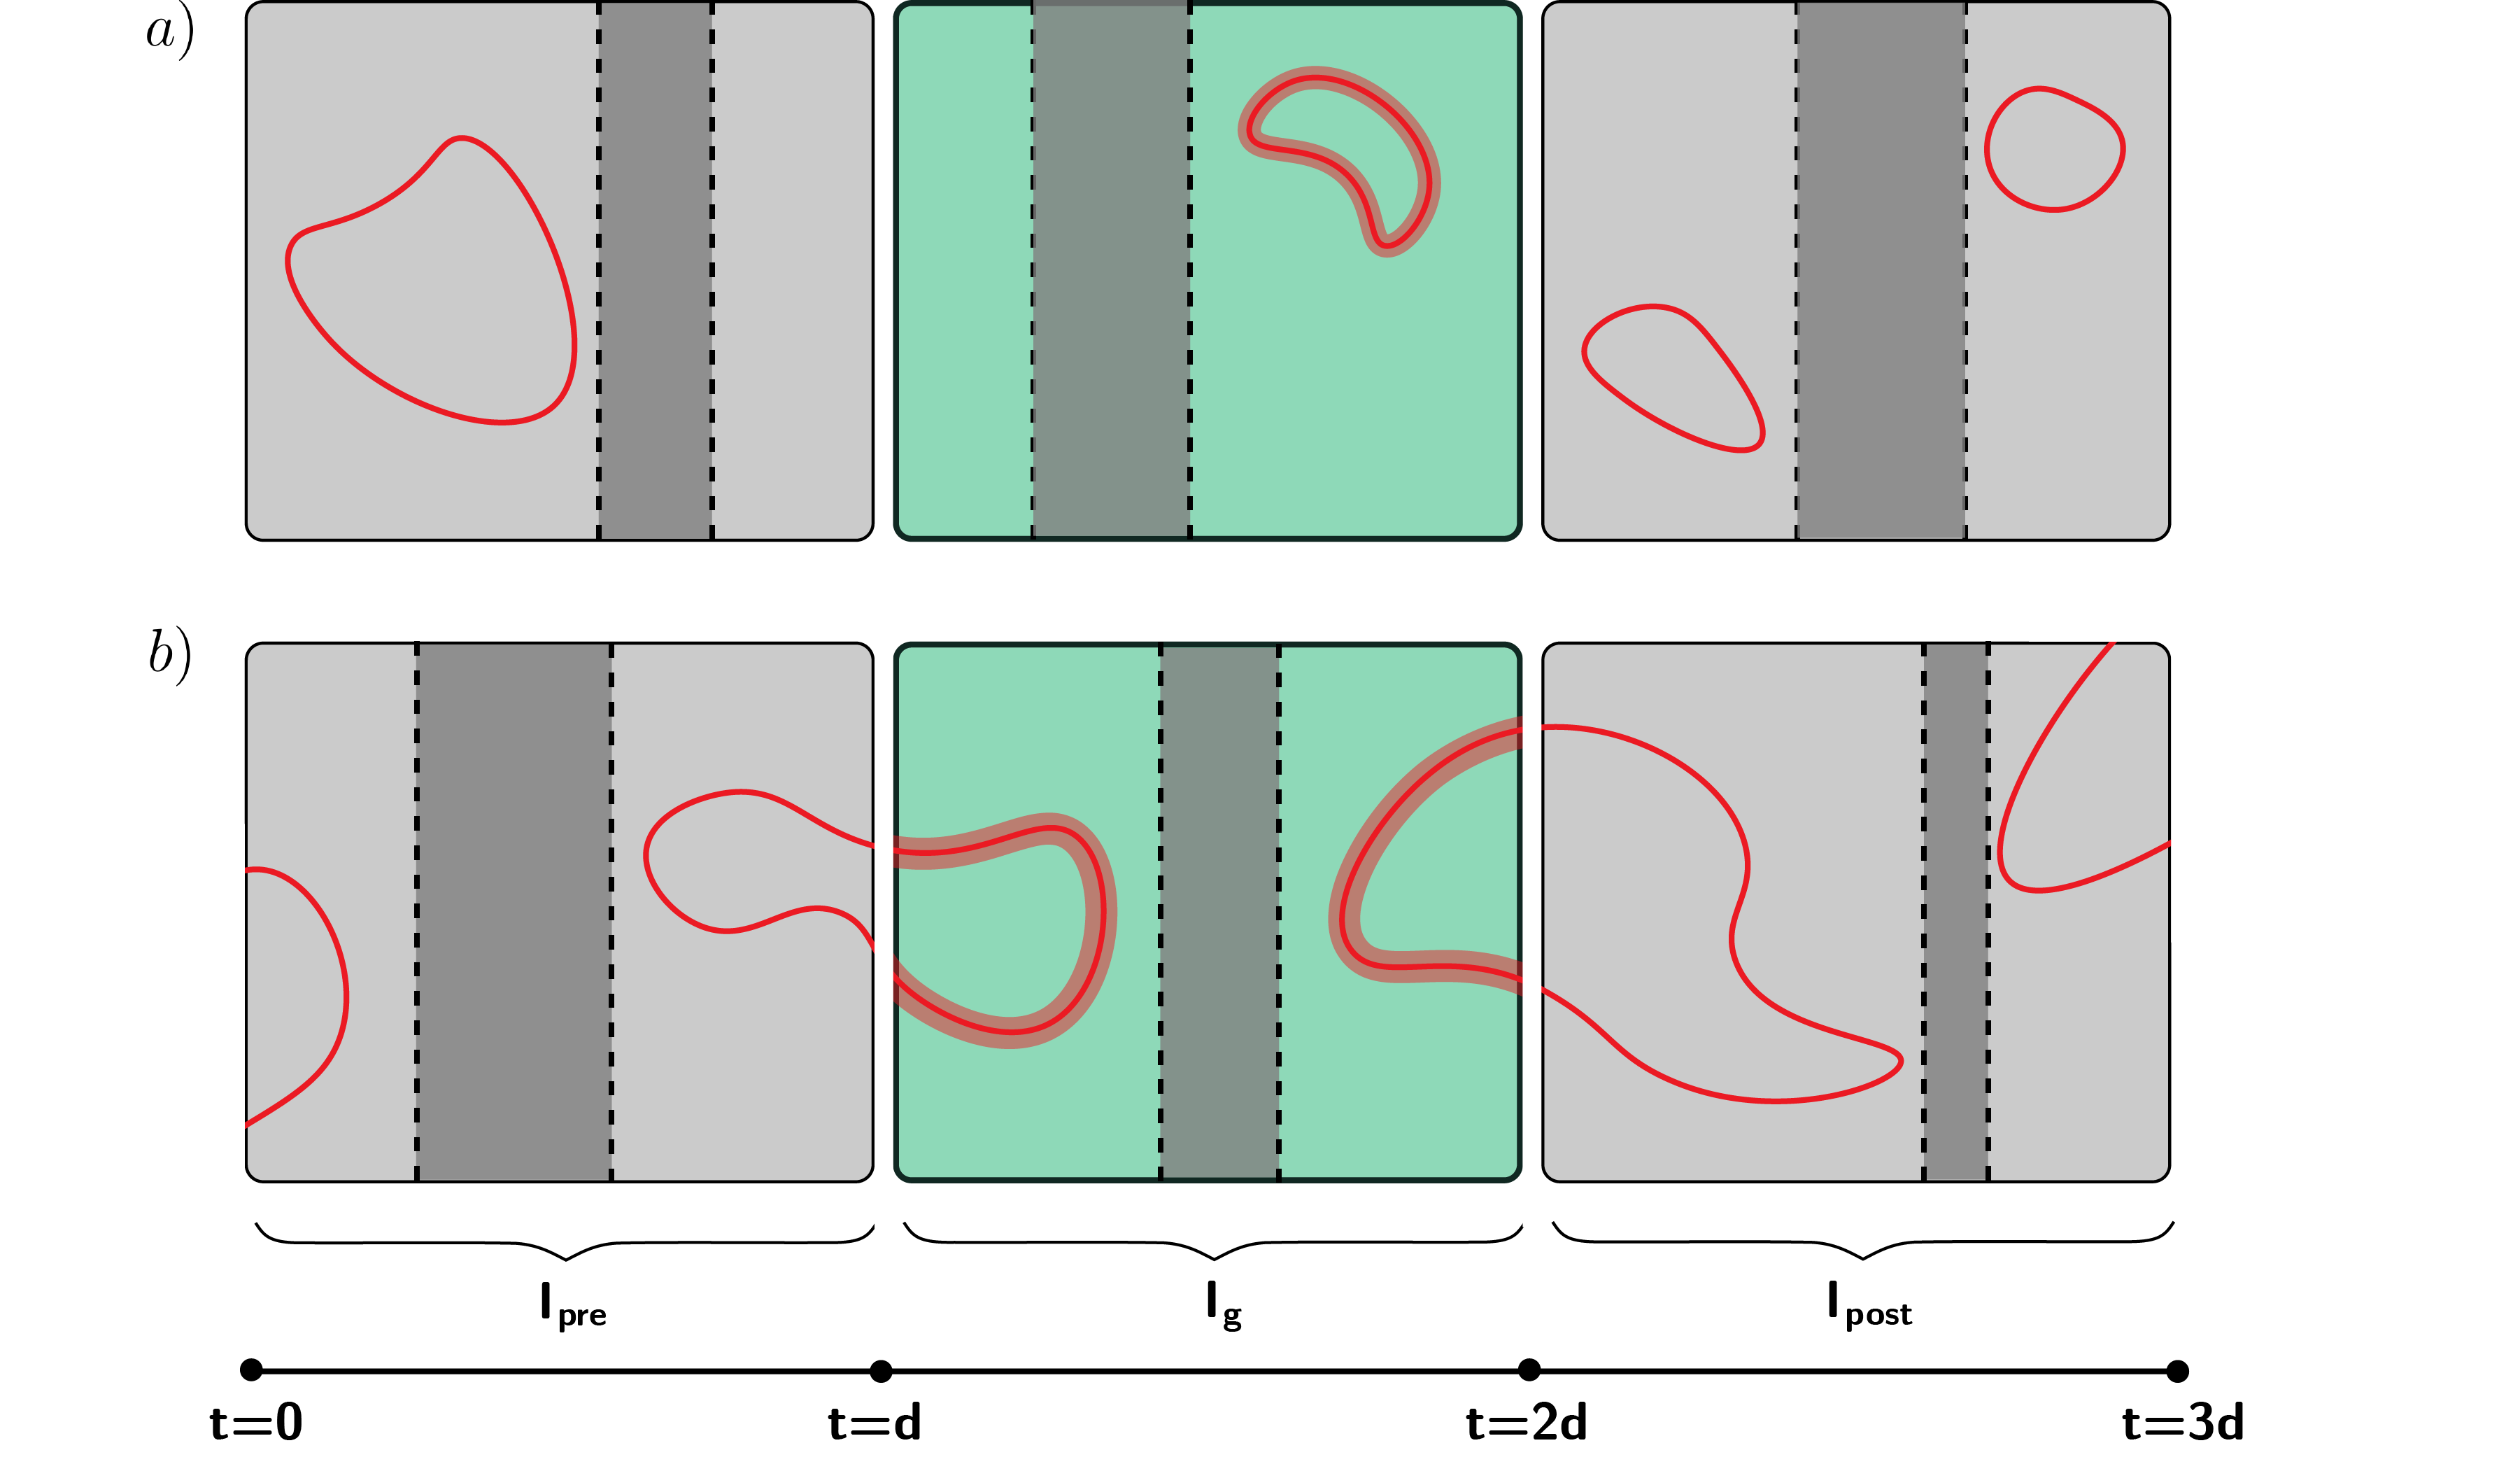
\includegraphics[width=0.75\linewidth]{figs/cutting-condition.png}
    \caption{Two different loop-like faults in spacetime that satisfy the cutting condition (Def. \ref{def:cutting-condition}). a) $P_\pm$ are the unshaded regions, while $C$ is the shaded region of spacetime where the faults have no support. In each of the three segments of the measurement protocol, pre-, during, and post-gauging, we can find a suitable region $C$. b) The cutting condition can hold for faults spanning gauging boundaries as well.}
    \label{fig:cutting-condition}
\end{figure}

\begin{lemma}[Existence of a cut]
\label{lem:cutting-condition-existence}
For some $1 < c_\mathrm{cut}=O(1)$, every loop-like fault configuration $F$ with $\Wt(F)<d/c_\mathrm{cut}$ has a clean cut for each of $I_\mathrm{pre}, I_\mathrm{g}, I_\mathrm{post}$.
\end{lemma}
\begin{proof}
Our strategy to prove the existence of a clean cut is to first break a given fault into connected components on the detector hypergraph. Given a large enough $c_{\rm cut}$, we are able to show that there must always be some interval of size $4 \upsilon$ between some pair of connected components. This interval can then define our clean cut. 

We know a loop-like fault must consist of some union of connected components--- other loop-like faults--- because it does not violate any (deterministic) detectors, and so must have no boundary on $\mathcal{H}$. Let the weight of a loop-like fault $F$ be $|F| \leq d/c_{\rm cut}$. We know that since $I_{\rm pre}, I_{\rm g}, I_{\rm post}$ all consist of $d$ time steps, there must be at least $d - d/c_{\rm cut}$ time steps \emph{without any faults}. 

We still need to demonstrate that there is a single interval between connected components of $F$ that has suitably large weight, say $4 \upsilon$. This ensures that the dropped detectors localized to a connected component also do not touch. 

In the worst case, the set of $d( 1- 1/c_{\rm cut})$ time steps without faults are spread out between many small connected components. In particular, say we have $d/c_{\rm cut}$ connected components, equally spaced. Then the number of time steps between each connected component is:
\[
\frac{d - d/c_{\rm cut}}{d/c_{\rm cut}} = c_{\rm cut} - 1 \geq 4 \upsilon \implies c_{\rm cut} \geq 4\upsilon + 1
\]
As $\upsilon = O(1)$, we can also find a suitable $O(1)$ $c_{\rm cut}$. Note that $c_{\rm cut} > 1$ always as well. 

We can then pick one interval in each of $I_{\rm pre}, I_{\rm g}, I_{\rm post}$ to perform the cut.

\end{proof}

If a fault satisfies the cutting condition, we are able to ``clean'' each portion of the fault on either side of the cut onto one of the temporal boundaries. 

\subsection{Cleaning} \label{sec:cleaning}

We now describe a process that can be applied to ``clean'' loop-like fault configurations that do not span the time direction of the protocol. Cleaning such a fault results in an equivalent fault that is supported completely at the gauging and ungauging time steps. 

More precisely, Lemma~\ref{lem:rewriting-abelian} and~\ref{lem:rewriting-non-abelian}, show how to rewrite Abelian and non-Abelian faults across one gauged round.
Def.~\ref{def:two-stage} combines these rewrite rules into a two-stage cleaning procedure to move all faults from one time step to the next, while Lemma~\ref{lem:cleaning-equivalence} proves the cleaning procedure is an exact re-writing of any given trajectory Kraus operator.
Def.~\ref{def:iter-cleaning} defines an iterated cleaning procedure to move all faults to one of the boundary rounds $t = 1, d+1, 2d+1, 3d$.

For a fault configuration $F$ and $d+2\le t\le 2d$, let
\[
F_t:=\{(t,f)\in F : (t,f) \text{ is a spatial fault}\}=F_t^A \sqcup F_t^N,
\]
where $F_t^A$ and $F_t^N$ are its Abelian and non-Abelian faults. 

Fix an order of the spatial faults at each time $t$ and let
\begin{align}
E_t(F) := \eta_t N_tA_t,\qquad A_t :=\prod_{(t,f)\in F_t^A}f_A,\qquad 
N_t:=\prod_{(t,f)\in F_t^N}f_N,
\label{eq:Et-At-Nt}
\end{align}
where $\eta_t \in \{\pm 1\}$ is the phase produced by this reordering.


\begin{lemma}[Rewriting Abelian faults across a gauged round]
\label{lem:rewriting-abelian}
    Let $(F,r)$ be a trajectory, 
    let $d+2\le t\le 2d$ and let $f_A$ be the Pauli operator of an elementary Abelian fault at time $t$ or $t+1$.
    For each $Q\in \cN \cup \cA$, define $\epsilon(f_A,Q)\in \{\pm 1\}$ by
    \[
        Qf_A = \epsilon(f_A,Q) f_A Q.
    \]
    In particular, $\epsilon(f_A,Q)=1$ for all $\nS{j}\in \cN$.
    Define 
    \[
    r^{(t,f_A)}(Q,t^*) :=
    \begin{cases}
        \epsilon(f_A,Q) r(Q,t),\qquad &t^*=t,\\
        r(Q,t^*),\qquad &t^*\neq t.
    \end{cases}
    \]
    Then,
    \begin{align}
        \label{eq:push-abelian-forward}
        M_t(r,r_F)f_A = f_A M_t(r^{(t,f_A)},r_F),\\
        \label{eq:push-abelian-backward}
        f_A M_t(r,r_F) = M_t(r^{(t,f_A)},r_F) f_A.
    \end{align}
    We refer to Eq.~\eqref{eq:push-abelian-forward} and Eq.~\eqref{eq:push-abelian-backward} as \emph{forward} and \emph{backward Abelian rewrites}, respectively.
\end{lemma}
\begin{proof}
    
    For every $Q\in \cN\cup \cA$, the definition of $\epsilon(f_A,Q)$ directly gives
    \begin{align}
    \label{eq:abelian-projector-commutator}
        \Pi_{r(Q,t)}f_A = f_A\Pi_{\epsilon(f_A,Q) r(Q,t)}.
    \end{align}
    Recall 
    \[
    M_t(r,r_F) = \bigl(\prod_{\mathbb{C}\in \cA_\kappa}\Pi_{r(\mathbb{C},t)}
    \bigr)\dots \bigl(\prod_{\mathbb{C}\in \cA_1}\Pi_{r(\mathbb{C},t)}
    \bigr)
    \bigl(\prod_{\mathbb{N}\in \cN} \Pi_{r(\mathbb{N},t)}
    \bigr)
    \]
    from Eq.~\eqref{eq:cases-M}.
    Using Eq.~\eqref{eq:abelian-projector-commutator}, compute 
    \begin{align}
        M_t(r,r_F)f_A&= \left(\prod_{C\in\cA_\kappa}\Pi_{r(C,t)}\right)\cdots\left(\prod_{C\in\cA_1}\Pi_{r(C,t)}\right)\left(\prod_{N\in\cN}\Pi_{r(N,t)}\right)f_A\\
        &=f_A\left(\prod_{C\in\cA_\kappa}\Pi_{r^{(t,f_A)}(\aS{},t)}\right)
        \cdots\left(\prod_{C\in\cA_1}\Pi_{r^{(t,f_A)}(\aS{},t)}\right)
        \left(\prod_{N\in\cN}\Pi_{r^{(t,f_A)}(\nS{},t)}\right)\\
        &=f_A M_t\bigl(r^{(t,f_A)},r_F\bigr).
    \end{align}
    Eq.~\eqref{eq:push-abelian-backward} follows from Eq.~\eqref{eq:push-abelian-forward}: since $\epsilon_{f_A,Q}^2 = 1$,  $(r^{(f_A,t)})^{(f_A,t)}=r$. Relabeling $r$ with $r^{(f_A,t)}$ and $r^{(f_A,t)}$ with $r$ in equation~\ref{eq:non-abelian-forward} gives Eq.~\eqref{eq:push-abelian-backward}.
\end{proof}

Thus, $f_A$ can be rewritten from round $t$ to $t+1$ (Eq.~\eqref{eq:push-abelian-forward}) or from round $t+1$ to round $t$ (Eq.~\eqref{eq:push-abelian-backward}) without changing its Pauli support.
During this move, the \textit{projected} history $r(Q,t)$ changes to $r^{(t,f_A)}$, while the \textit{recorded} history remains $r_F$.
In order for measured outcomes $r_F$ to remain the same despite the changed eigenspace projections at round $t$, the fault configuration needs to change. In particular, measurement errors are added at round $t$. Changing these measurement errors while pushing these Abelian faults between rounds is analogous to multiplying by Pauli spacetime stabilizers in standard spacetime cleaning methods in Pauli stabilizer codes.

We later compose these rewrites iteratively over many rounds. This requires us to bound the number of spatial and temporal faults changed by each rewrite, since the final cleaned configuration need not have $O(\Wt(F))$ if we are not careful.

\begin{corollary}[Fault support and weight after Abelian rewrites]
\label{cor:fault-support-abelian-rewrite}
    
    Each Abelian rewrite in in Lemma~\ref{lem:rewriting-abelian} does not change the support of $f_A$.
    Further, recorded history remains $r_F$. 
\end{corollary}
\begin{proof}
    The same Pauli operator $f_A$ appears on both sides of equations~\eqref{eq:push-abelian-forward} and~\eqref{eq:push-abelian-backward}. Only the time at which it occurs changes. Thus, the number of elementary spatial faults and the qubit support of the spatial fault is unchanged after the rewrite.
    
    Now we show that the Abelian rewrite can keep the $r_F$ measurement outcome history the same by changing only $O(1)$ measurement events in round $t$.
    It suffices to only examine $\cA$ checks because $f_A$ rewrites do not change the projected eigenspaces of $\cN$ checks.
    For each $\aS{i}\in \cA$, let $\pi_{i}$ be the temporal fault permutation at $(\aS{i},t)$. Take $\pi_{\aS{i}}=\id$ when no temporal fault occurs. 
    Replace the temporal fault permutation $\pi_i$ by the permutation $\pi_i'$ defined by
    \[
    \pi_{i}'(\epsilon(f_A,\aS{i})\lambda ):= \pi_i {\lambda},\qquad \lambda\in \lambda(\aS{i}).
    \]
    This defines a permutation where multiplication by $\epsilon(f_A,\aS{i})$ permutes $\lambda(\aS{i})$.
    Then,
     \begin{align}
         \pi_i'(r^{(t,f_A)}(\aS{i},t)) &= \pi_i'(\epsilon_i r(\aS{i},t))\\
        &=\pi_i( r(\aS{i},t))\\
        &=r_F(\aS{i},t).
     \end{align}
    Thus the recorded history $r_F$ is unchanged.
    Moreover, $\pi_i=\pi_i'$ when $\epsilon_i=1$. Since $f_A$ is local, and the measured checks have bounded qubit degree, these permutations change at only $O(1)$ measurement events.    
\end{proof}

Moving an elementary non-Abelian fault through a measurement projector (see Fact.~\ref{fact:moving-nonabelian}) can change the projected eigenvalue and produce a linear combination of Abelian byproducts.
To track the operators produced by compositions of these rewrites, we introduce the following error space containing all possible products and linear combinations of a set of elementary spatial faults.
Below, we apply this definition to the Abelian byproducts generated by the non-Abelian rewrites (Lemma~\ref{lem:rewriting-non-abelian}).

\begin{definition}[Error space generated by faults]
    For a finite set $R$ of elementary spatial faults, define 
    \[
    \mathrm{Err}(R) := \rm{span}\Biggl\{\prod_{(t,f)\in R'} f:R'\subseteq R\Biggr\}
    \]
    where every product is taken in a fixed order of the spatial faults $f$, and an empty product is $\id$.
    Thus, $\mathrm{Err}(R)$ contains linear combinations of products of the faults in $R$.

    We use the same notation $\mathrm{Err}(S)$ for a set of spatial locations.
    If $S\subseteq \mathsf{L}_\mathrm{s}$, whose elements are the spatial locations $(t,\vertexset{v})$ and $(t,\{e\})$ from Def.~\ref{def:fault-location-hypergraph}, 
    define
    \[
    \mathrm{Err}(S) := \mathrm{Err}(\{(t,f)\in \Lambda: \exists (t,l)\in S, \supp{f}\subseteq l\}).
    \]
\end{definition}

For every $(t,f_N)\in F_t^N$, $\aS{}\in \cA$, and $\diamond\in \{\leftarrow, \rightarrow\}$, fix the ordered factorization in Lemma~\ref{lem:byproducts},
\begin{align}
\label{eq:b-arrow-factorization}
    B_\diamond(f_N,\aS{}) = f_{A,1}^\diamond(f_N,\aS{})\dots f_{A,m}^\diamond(f_N,\aS{})\ \text{up to a phase},\qquad m\le \beta,
\end{align}
where each $f_{A,j}^\diamond(f_N,\aS{})$ is the Pauli operator of an elementary Abelian fault at time $t$.

Define 
\[
\cB_t:=\{(t,f_{A,j}^{\diamond}(f_N, \aS{})):(t,f_N)\in F_t^N,\ \aS{}\in \cA,\  \diamond\in \{\rightarrow, \leftarrow\},\ 1\le j\le m,\ f_{A,j}^\diamond(f_N, \aS{})\neq \id\}.
\]
This is the set of all nonidentity elementary Abelian byproducts that can arise when non-Abelian faults in $F_t^N$ are moved, in either direction, through the $\cA$-projectors measured in round $t$.

\begin{lemma}[Rewriting non-Abelian faults across a round in the gauged code]
\label{lem:rewriting-non-abelian}
Let $(F,r)$ be a trajectory. For $d+2 \le t \le 2d$, moving $N_t$ forward to round $t+1$ across $M_t$ gives 
\begin{align}
    M_t(r,r_F) N_t &= N_t \left(\sum_j M_t(r_j, r_F) A_j\right),\qquad A_j\in \mathrm{Err}(\cB_t).\label{eq:non-abelian-forward}
\end{align}
For $d+2 \le t \le 2d-1$, moving $N_{t+1}$ backwards to round $t$ across $M_t$ gives
\begin{align}
    N_{t+1} M_t(r,r_F) &= \left(\sum_j A_j' M_t (r_j',r_F)\right) N_{t+1},\qquad A_j'\in \mathrm{Err}(\cB_{t+1}).\label{eq:non-abelian-backward}
\end{align}
Every $r_j(Q,t^*)$ and $r_j'(Q,t^*)$ is an outcome function that agrees with $r(Q,t^*)$ for $t^*\neq t$.
Moreover, every term has the same recorded term $r_F$.
We refer to Eq.~\eqref{eq:non-abelian-forward} and Eq.~\eqref{eq:non-abelian-backward} as \emph{forward} and \emph{backward non-Abelian rewrites}, respectively.
\end{lemma}
\begin{proof}
    Write
    \[
    N_t = f_{N,s}\dots f_{N,1},\qquad M_t =P_{l}\dots P_1
    \]
    using a fixed fault order and a fixed order of the projectors at round $t$ (Eq.~\eqref{eq:cases-M}). We use $P_\ell$ with subscript $1\le \ell \le l$ to enumerate the projectors in $M_t$.
    
    Suppose $P_\ell=\Pi_{\mu}$ projects onto an 
    $\nS{}\in \cN$ eigenspace with eigenvalue $\mu$, 
    then the fact that both $\nS{}$ and $f_{N,k}$ ($1\le k\le s$) are Pauli means that $\nS{}f_{N,k}=\epsilon f_{N,k}\nS{}$ for some $\epsilon\in \{\pm 1\}$,
    and thus
    \begin{align}
    \label{eq:move-non-abelian-projector}
        \Pi_{\mu} f_{N,k} = f_{N,k}\Pi_{\epsilon \mu}.
    \end{align}
    Now suppose that $P_\ell=\Pi_{\mu}$ instead projects onto a $\aS{}\in \cA$ eigenspace. Abbreviate $O_\leftarrow:= \aS{}B_\leftarrow(f_{N,k},\aS{}) \aS{}^\dagger$ and $O_\rightarrow:=B_\rightarrow (f_{N,k},\aS{})$.
    Fact~\ref{fact:moving-nonabelian} directly gives forward and backward rewrites for an elementary non-Abelian fault across an Abelian projector: 
    \begin{align}
        \Pi_{\mu}f_{N,k} = f_{N,k}\sum_{\epsilon=\pm1} \Pi_{\epsilon \mu} 
        \frac{\id + \epsilon O_\leftarrow}{2}
        \label{eq:forward-elementary-non-abelian}\\
        f_{N,k}\Pi_{\mu}=
        \sum_{\epsilon=\pm1}
        \Pi_{\epsilon \mu}
        \frac{\id + \epsilon O_\rightarrow}{2}f_{N,k}.
        \label{eq:backward-elementary-non-abelian}
    \end{align}

    First we observe that $O_\leftarrow,O_\rightarrow\in\mathrm{Err}(\cB_t)$. To see this, recall that each $B_\leftarrow (f_{N,k},\aS{})$ has a fixed factorization (Eq.~\eqref{eq:b-arrow-factorization})
    \[
    B_\leftarrow (f_{N,k},\aS{}) = \omega_{\leftarrow}\prod_if_{A,i}^{\leftarrow},
    \]
    where we have abbreviated $f_{A,i}^\leftarrow = f_{A,i}^\leftarrow(f_{N,k},\aS{})$.
    $(t,f_{A,i}^\leftarrow)\in \cB_t$ and $\omega_\leftarrow$ is a phase. 
    Every $f_{A,i}^\leftarrow$ is an elementary Abelian spatial fault, $\aS{}f_{A,i}^{\leftarrow} \aS{}^{\dagger}=\eta_i f_{A,i}^{\leftarrow}$ for some $\eta_i\in \{\pm 1\}$.
    Therefore,
    \[
    O_\leftarrow = \omega_\leftarrow \bigl(\prod_{i}\eta_i \bigr) \prod_i f_{A,i}^\leftarrow \in \mathrm{Err}(\cB_t).
    \]
    The same calculation with $B_\rightarrow$ gives $O_\rightarrow\in \mathrm{Err}(\cB_t)$.

    After one forward rewrite, Eq.\eqref{eq:forward-elementary-non-abelian} when expanded is
    \[
    \Pi_\mu f_{N,k} = \frac{1}{2}f_{N,k} (\Pi_\mu + \Pi_{-\mu} + \Pi_\mu O_\leftarrow - \Pi_{-\mu} O_\leftarrow).
    \]
    Moving an elementary non-Abelian fault through the $\aS{}$ measurement produces trajectories with either projected history $\mu$ or $-\mu$. Additionally, this move results in a linear combination of Abelian byproducts to the right of the projector $\Pi_{\epsilon \mu}$, $(\id\pm \epsilon O_\leftarrow)$, which depends on the projected eigenspace.

    Now apply Eqs.~\eqref{eq:move-non-abelian-projector},~\eqref{eq:forward-elementary-non-abelian} and~\eqref{eq:backward-elementary-non-abelian} successively to the factors of $N_t = f_{N,s}\dots f_{N,1}$, and sequentially move each $f_{N,k}$ to the left of $M_t$ from $f_{N,s}$ to $f_{N,1}$.
    When moving $f_{N,k}$ past a non-Abelian projector, we change the sign of the projected eigenspace, as in Eq.~\eqref{eq:move-non-abelian-projector}. When moving $f_{N,k}$ past an Abelian projector, we use Eq.~\eqref{eq:forward-elementary-non-abelian} and~\eqref{eq:backward-elementary-non-abelian}.
    Each time a non-Abelian fault is moved past an Abelian projector, it replaces the current term in the sum with four terms: the projected eigenspace is either $\mu$ or $-\mu$, and the factor to the right of the projector is either $\id$, $O_\leftarrow$, or $-O_\leftarrow$. 
    We continue until every factor of $N_t$ has been moved to the left of every projector in $M_t$. Let $j$ label one non-zero term in this finite sum. By definition, once a $j$ is fixed, so are all projectors $P_{\ell,j}$ ($1\le \ell \le l$, $\ell\in \mathbb{N}$) and Abelian faults between these projectors $A_{\ell,j}$. We include any factors of $1/2$ and other commutation signs in $A_{\ell,j}$.
    Presently, we have
    \[
    M_t(r,r_F)N_t = N_t \sum_{j} P_{l,j}  A_{l,j}\dots P_{1,j}A_{1,j},\qquad A_{\ell,j}\in \mathrm{Err}(\cB_t).
    \]
    Every $A_{\ell,j}\in \mathrm{Err}(\cB_t)$ because it is a scalar multiple of a product of generated elementary Abelian byproducts.

    We apply the backward Abelian rewrite (Lemma~\ref{lem:rewriting-abelian}) to each term labeled by $j$ to put all $A_{\ell,j}$ to the right of $M_t$:
    \[
    M_t(r,r_F)N_t = N_t \sum_{j} P_{l,j}  A_{l,j}\dots P_{1,j}A_{1,j}= 
    N_t\sum_j M_t(r_j,r_F)A_j
    \qquad A_j\in \mathrm{Err}(\cB_t) 
    \]
    Thus we have exactly Eq.~\eqref{eq:non-abelian-forward} in the claim. Starting instead with Eq.~\eqref{eq:backward-elementary-non-abelian} and following the same argument with $O_\rightarrow$ instead of $O_\leftarrow$ gives Eq.~\eqref{eq:non-abelian-backward}.
\end{proof}


\begin{corollary}[Fault support and weight after non-Abelian rewrites]
\label{cor:fault-support-non-abelian-rewrites}
    In the forward (backward) non-Abelian rewrite in Eq.~\eqref{eq:non-abelian-forward} (Eq.~\eqref{eq:non-abelian-backward}), every $A_j$ \emph{($A_j'$)} is a scalar multiple of a product of at most $O(|F_t^N|)$ \emph{($O(|F_{t+1}^N|)$)} elementary Abelian spatial faults at time $t$ \emph{($t+1$)}.
\end{corollary}
\begin{proof}
    Each elementary non-Abelian fault intersects $O(1)$ measured checks.
    When we sequentially move each non-Abelian elementary fault in $F_t^N$ ($F_{t+1}^N$) during the forward (backward) rewrite, the elementary fault non-trivially overlaps with $O(1)$ projectors. 
    
    Thus, we invoke Fact~\ref{fact:moving-nonabelian} only $O(|F_t^N|)$ ($O(|F_{t+1}^N|)$) times.
    Each use of Fact~\ref{fact:moving-nonabelian} produces at most $\beta = O(1)$ elementary Abelian factors by Lemma~\ref{lem:byproducts}. 
    We then must have that the total number of elementary Abelian byproducts produced by moving $F_t^N$ ($F_{t+1}^N$) across $M_t$ is at most $O(|F_t^N|)$ ($O(|F_{t+1}^N|)$).
    
    Using the Abelian rewrite rule (Lemma~\ref{lem:rewriting-abelian}) to move all Abelian byproducts to the right (left) of $M_t$ keeps the same spatial support and number of elementary Abelian faults by Lemma~\ref{cor:fault-support-abelian-rewrite}. 
    Therefore, every product $A_j$ ($A_j'$) contains at most $O(|F_t^N|)$ ($O(|F_{t+1}^N|)$) elementary Abelian faults at time $t$ ($t+1$).
    
\end{proof}

\begin{definition}[Two-stage cleaning across one time step]
\label{def:two-stage}
    Let $(F,r)$ be a trajectory, and let $M_t$ be the stabilizer measurements in round $t$.

    Let $d+2\le t\le 2d$.
    To clean spatial faults at time $t$ forward to time $t+1$,
    \begin{enumerate}
        \item Apply the forward non-Abelian rewrite in Lemma~\ref{lem:rewriting-non-abelian}. This moves $F_t^N$ from time $t$ to $t+1$, and leaves Abelian byproducts at time $t$. The trajectory $(F,r)$ is expanded into a sum of many trajectories, $(F_j,r_j)$, each with the same noisy outcome history $r_F$.
        \item For each $(F_j,r_j)$ trajectory in the expansion, use the forward rewrite in Lemma~\ref{lem:rewriting-abelian} to move every original fault in $F_t^A$ and all Abelian byproducts across $M_t$ to round $t+1$.
    \end{enumerate}
    We refer to the above procedure as \emph{forward two-stage cleaning}.

    Let $d+2\le t\le 2d-1$.
    To clean spatial faults at time $t+1$ backwards to time $t$,
    \begin{enumerate}
        \item Apply the backward non-Abelian rewrite in Lemma~\ref{lem:rewriting-non-abelian}. This moves $F_{t+1}^N$ from time $t+1$ to $t$, and leaves Abelian byproducts at time $t+1$. The trajectory $(F,r)$ is expanded into a sum of many trajectories, $(F_j,r_j)$, each with the same noisy outcome history $r_F$.
        \item For each $(F_j,r_j)$ trajectory in the expansion, use the backwards rewrite in Lemma~\ref{lem:rewriting-abelian} to move every original fault in $F_{t+1}^A$ and all Abelian byproducts across $M_t$ to round $t$.
    \end{enumerate}
    We refer to the above procedure as \emph{backward two-stage cleaning}.
\end{definition}

\begin{lemma}[Cleaning equivalence]
\label{lem:cleaning-equivalence}
    Let $(F,r)$ be a trajectory, and perform a forward two-stage cleaning or a backwards
    two-stage cleaning (Def.~\ref{def:two-stage}). The resulting sum of trajectories $(F_j,r_j)$ and coefficients $\alpha_j\in \mathbb{C}$ satisfy
    \[
    K(F,r) = \sum_j \alpha_j  K(F_j,r_j),\ \qquad (r_j)_{F_j} = r_F
    \]
    for every non-zero term. $(r_j)_{F_j}$ denotes the recorded history computed from $r_j$ and $F_j$.
    Thus, the two-stage cleaning is an exact rewrite of the Kraus operator corresponding to the trajectory $(F,r)$ and it does not change the recorded outcome history.
\end{lemma}
\begin{proof}
    We first prove the claim for forward two-stage cleaning by applying the exact operator identities in lemmas~\ref{lem:rewriting-abelian} and~\ref{lem:rewriting-non-abelian}.
    Let us write the Kraus operator for the $(F,r)$ trajectory as
    \[
        K(F,r) = K_{>t}(F,r)M_t(r,r_F) E_t(F) K_{<t}(F,r),
    \]
    where 
    \[
    K_{>t}(F,r):= M_{3d}E_{3d}\dots M_{t+1}E_{t+1},\qquad
    K_{<t}(F,r):= M_{t-1}E_{t-1}\dots M_1E_1,
    \]
    we have dropped the $(F,r)$ arguments for readability.
    Using Eq.~\eqref{eq:Et-At-Nt} and the forward non-Abelian rewrite, 
    \begin{align}
        K(F,r) &= \eta_t K_{>t} M_t(r,r_F)N_t A_t K_{<t}\notag\\
        &= \eta_t K_{>t} N_t \bigl( \sum_{j}M_{t}(r_j,r_F)A_j\bigr) A_t K_{<t}.
    \end{align}
    Expand each $A_j\in \mathrm{Err}(\cB_t)$ as $A_j\in \sum_a c_{j,a}G_{j,a}$ where $G_{j,a}$ is a product of elementary Abelian byproducts.
    Applying the forward Abelian rewrite in Lemma~\ref{lem:rewriting-abelian} to the factors of $G_{j,a}A_t$ alters the projected outcome,
    \[
    M_t(r_j,r_F) G_{j,a} A_t = G_{j,a} A_t M_t(r_{j,a}, r_F).
    \]
    Thus, we presently have
    \[
    K(F,r) = \sum_{j,a} \eta_t c_{j,a} K_{>t} N_t G_{j,a} A_t M_{t}(r_{j,a},r_F) K_{<t}.
    \]
    In each term in the sum, the spatial faults that were formerly at time $t$, and all their spatial Abelian byproducts, now occur at time $t+1$.
    We collect them all and the rest of the faults in $F$ into a fault configuration $F_{j,a}$, and absorb the scalar coefficients into $\alpha_{j,a}$.
    Finally, we have 
    \[
    K(F,r) = \sum_{j,a} \alpha_{j,a} K(F_{j,a},r_{j,a}).
    \]

    For the backward rewrite, it is convenient to first reorder the Abelian and non-Abelian factors in $E_{t+1}(F)$ to $E_{t+1}(F) =\eta_t' A_{t+1}N_{t+1}$, so that $N_{t+1}$ is adjacent to $M_t$.
    Since both operators are Pauli, this only introduces an overall sign absorbed into the scalar coefficient.
    The backward non-Abelian and Abelian rewrites then give the same expansion in the claim, with all spatial faults moved to time $t$.

    The projected outcome function changes twice during this calculation: the non-Abelian move replaces $r$ by $r_j$ and the subsequent Abelian moves replace $r_j$ by $r_{j,a}$. Both changes only occur at measurement events in round $t$.
    To keep the recorded outcome history, $r_F$, the same for all trajectories $(F_{j,a},r_{j,a})$, replace the temporal fault permutation at each changed measurement event $(Q,t)$ by a permutation $\pi_{j,a,Q}$ that satisfies
    \[
    \pi_{j,a,Q}\bigl(r_{j,a}(Q,t)\bigr) = r_F(Q,t).
    \]
    At every unchanged measurement event, we keep the same distribution of temporal faults as $F$.
    It follows that \[
    (r_{j,a})_{F_{j,a}} = r_F
    \]
    at every measurement event, for all trajectories $(F_{j,a},r_{j,a})$.
    Replacing the double index $j,a$ with a single index $j$ shows the claimed result.    
\end{proof}

\begin{remark}[Cleaned trajectories remain loop-like]
    Note, since the observed outcomes $r_{F_j}=r_F$ are preserved under cleaning, if we begin with a loop-like fault $F$, all resulting trajectories $F_j$ will be loop-like as well.
\end{remark}

\begin{corollary}[Fault support and weight after two-stage cleaning]
\label{cor:two-stage-fault-support}
For every nonzero term $\alpha_jK(F_j,r_j)$ in the expansion produced by forward two-stage cleaning across $M_t$,
\begin{enumerate}
    \item No spatial faults remain at time $t$, so $(F_j)_t=\emptyset$;
    \item the spatial faults at the destination time $t+1$ satisfy \[
    |(F_j)_{t+1}| \le |F_{t+1}| + c_{\rm{clean}}|F_t|
    \]
    for a constant $c_{\rm{clean}}=O(1)$;
    \item $F_j$ and $F$ have the same spatial faults at every time
    $t^*\notin\{t,t+1\}$; and
    \item $F$ and $F_j$ differ by at most $O(|F_t|)$ measurement events in round $t$.
\end{enumerate}
These claims hold for backward two-stage cleaning after interchanging $t$ and $t+1$ and replacing $F_t$ with $F_{t+1}$.
\end{corollary}
\begin{proof}
    Consider forward cleaning.
    By Lemma~\ref{cor:fault-support-non-abelian-rewrites}, the forward non-Abelian rewrite moves all faults in $F_t^N$ across $M_t$ and generates at most $c_N|F_t^N|$ elementary Abelian byproducts in every resulting trajectory, for a constant $c_N=O(1)$.
    The subsequent forward Abelian rewrites move these byproducts and every fault in $F_t^A$ across $M_t$. Hence, every spatial fault originally at time $t$, which is the union $F_t^N\cup F_t^A$, and any byproducts generated by moving these faults occur at time $t+1$ after two-stage cleaning. This proves that $(F_j)_t=\emptyset$.
    
    Now we consider all spatial faults at time $t+1$ after two-stage cleaning.
    The faults newly placed at time $t+1$ consist of the original $|F_t|$ faults and at most $c_N|F_t^N|$ byproducts. Together with the faults that were already at $F_{t+1}$ from the original fault configuration $F$,
    \begin{align}
        |(F_j)_{t+1}| &\le |F_{t+1}| + |F_t| + c_N|F_t^N|\notag\\
        &\le |F_{t+1}| + (1 + c_N)|F_t| .
    \end{align}
    Thus the second claim holds for $c_{\mathrm{clean}}:=(1+c_N)=O(1)$. Any overlapping faults in $F_{t+1}$ that happen to cancel out on their support only decrease the left hand side of this inequality.

    Both stages in the two-stage cleaning only rewrite the faults at times $t$ and $t+1$. They therefore leave the spatial faults at every time $t^*\notin \{t,t+1\}$ unchanged from $F$, which is the third claim.

    Finally, the forward non-Abelian rewrite changes temporal faults at $O(|F_t^N|)$ measurement events at round $t$, by Lemma~\ref{cor:fault-support-non-abelian-rewrites}.
    There are at most $|F_t^A|+c_N|F_t^N| = O(|F_t|)$ Abelian faults and byproducts that are moved in the second stage of the two-stage cleaning. Each forward elementary Abelian rewrite changes temporal faults at $O(1)$ round $t$ measurement events by Lemma~\ref{cor:fault-support-abelian-rewrite}; moving $O(|F_t|)$ elementary Abelian faults in $t$ changes $ O(|F_t|)$ round $t$ measurement events.
    Thus, $F_j$ differs from $F$ at only $O(|F_t|)$ temporal locations, all in round $t$.

    For backwards cleaning, the same arguments apply to all faults in $F_{t+1}$ by interchanging $t$ and $t+1$ in the first three claims. 
\end{proof}

\begin{remark}[Weight after iterating two-stage cleaning]
    Note that the weight of a cleaned fault does not grow exponentially with the number of rounds we have cleaned it through; the byproducts that may be produced by some non-Abelian elementary fault are always the same, since the stabilizers being measured each round are the same. Thus the spatial support of byproducts remains restricted to a bounded neighborhood around the fault as we move the fault through time, and thus the total byproduct weight remains bounded as well.
\end{remark}


For the next step of the cleaning, we need to consider what happens when we move faults through the gauging boundaries at $t=d+1$ and $t=2d+2$. We will first clean everything near the ungauging boundaries into the gauged code to produce a loop-like fault near $t=d+2$ and $t=2d+1$. Then, after proving the bounded weight of these remnant loop-like excitations, it will be most convenient to move them back into the base code to map the whole trajectory onto a completely deterministic set of detectors. 

When we are considering the boundary rewrites into the gauged code, there are three kinds of errors to consider: (i) Abelian matter faults, (ii) non-Abelian matter faults, and (iii) initialization/measurement errors on the edge ancilla. The following lemma describes the re-write rules across the gauging and ungauging boundaries:

\begin{lemma}[Boundary rewrites into the gauged code]
\label{lem:boundary-rewrites-into-gauged-code}
The boundary re-writes we need to consider are as follows.
\begin{itemize}
    \item Abelian matter faults: Abelian rewrites (Lemma \ref{lem:rewriting-abelian}) are unchanged across the boundary from the base code to the ungauged code as compared to the bulk of the gauged code.
    \begin{equation}
        M_{d+1}(r, r_F) A_{d+1} = A_{d+1} M_{d+1}(r^{(A_{d+1}, d+1)}, r_F)
    \end{equation}
    \begin{equation}
        A_{2d+2} M_{2d+1}(r, r_F) = \alpha(z) M_{2d+1}(r^{(f_A, 2d+1)}, r_F) A_{2d+2}
    \end{equation}
    Here, $\alpha(z) = A_{2d+2} U_{c(z)} A_{2d+2}^\dagger U_{c(z)}^\dagger$.
    \item non-Abelian matter faults: as with the bulk rewrites, non-Abelian faults generate Abelian byproduct operators when they pass from the base code to the gauged code.
    \begin{equation}
       M_{d+1}(r,r_F) N_{d+1} = N_{d+1} \left(\sum_j M_{d+1}(r_j, r_F) A_j\right),\qquad A_j\in \mathrm{Err}(\cB_{d+1})
    \end{equation}
    \begin{equation}
        N_{2d+2} M_{2d+1}(r, r_F) = M_{2d+1}(r^{(2d+1, N)}, r_F) B_{\rm bd.} N_{2d+2}
    \end{equation}
    Here, $B_{\rm bd.} = U_{c(z)}^\dagger N_{2d+2} U_{c(z)} N_{2d+2}^\dagger$.
    \item Initialization/readout errors on edge qubits: Ancilla initialization errors into non-Abelian faults when we push them onto the gauged code. 
    \begin{equation}
        M_{d+1}(r, r_F) \Xp_{d+1} = \Xp_{d+1} \left(\sum_j M_{d+1}(r_j, r_F) A_j\right),\qquad A_j\in \mathrm{Err}(\cB_{d+1}).
    \end{equation}
    Readout errors are already equivalent to non-Abelian errors on the gauged code, so we don't need to do anything to them.

    All boundary rewrites preserve the recorded history $r_F$.

\end{itemize}
    
\end{lemma}
\begin{proof}
    The two boundary times are $t = d+1$ and $t = 2d +1$. We want to push faults occurring just after we measure the base code stabilizers for the final time at $t=d+1$, onto the next slice where we have begun measuring the gauged code stabilizers at $t = d+2$. Likewise, we want to push any faults on the first time slice after returning to the base code, $t = 2d+2$, onto the time slice $t = 2d+1$ right after we have measured the gauged code stabilizers for the last time.

    Consider a fault configuration $F$, and let $A_{d+1}$ be the Abelian faults of $F$ acting on the base code at time $t=d+1$. By definition, each elementary Abelian Pauli fault must commute or anti-commute with the \emph{gauged} Abelian stabilizers. There is a stabilizer of the original code for every stabilizer $\mathbb{C} \in \cA \backslash \{\av\}$. The only difference between the decorated stabilizers $\mathbb{C}$ and the equivalent base code stabilizers is $\Zp$ support on the gauge qubits, thus an Abelian error supported on the matter qubits has the same commutation relations with $\mathbb{C}$ and its representative on the gauged code. Thus, the re-write rule across the boundary is identical to the usual Abelian re-write inside the gauged code.
    \begin{align}
        M_{d+1}(r, r_F) A_{d+1} = A_{d+1} M_{d+1}(r^{(A_{d+1}, d+1)}, r_F) \notag
    \end{align}
    Any projector values $r^{(A_{d+1}, d+1)}$ that are changed by passing $A_{d+1}$ through should have their assigned permutation flipped to ensure $r_F$ remains the same (as in Corollary \ref{cor:fault-support-abelian-rewrite}).
    
    Now consider all Abelian faults $A_{2d+2}$ at time $t = 2d+2$. The faults must be pushed backwards through the feedback circuit $U_{c(z)}$. Note that the action of $U_{c(z)}$ is identical to some product of the $\av$ operators when restricted to the matter qubits. As the $\av$ are Abelian stabilizers, $A_{2d+2}$ may only commute or anti-commute with them. Commuting $A_{2d+2}$ through $U_{c(z)}$ thus produces a global phase $\alpha(z)$. We retrieve the usual Abelian rewrite rule again, but up to this phase $\alpha(z)$.
    \begin{align}
        A_{2d+2} M_{2d+1}(r, r_F) = \alpha(z) M_{2d+1}(r^{(f_A, 2d+2)}, r_F) A_{2d+2} \notag 
    \end{align}
    Again, we also perform the necessary changes to the measurement faults to ensure $r_F$ is unchanged.

    Now consider all non-Abelian faults $N_{d+1}$ (supported on the matter degrees of freedom) on the base code at time $t=d+1$. We simply start measuring the gauged code stabilizers at $t=d+1$, so the re-write rules are exactly the same as the ones in Lemma \ref{lem:rewriting-non-abelian}.
    \[
    M_{d+1}(r,r_F) N_{d+1} = N_{d+1} \left(\sum_j M_{d+1}(r_j, r_F) A_j\right),\qquad A_j\in \mathrm{Err}(\cB_{d+1}).
    \]
    Here, $\cB_{d+1}$ should be understood as the set of all Abelian byproducts that arise when $N_{d+1}$ is pushed through the Abelian stabilizer measurements in time step $d+1$.
    
    For all non-Abelian faults $N_{2d+2}$ (supported on the matter degrees of freedom) on the base code, we must push them through the last round of base code syndrome measurements and the feedback circuit $U_{c(z)}$. Restricting any non-Abelian stabilizer of the gauged code onto the matter qubits yields either identity ($\bp$ stabilizers) or a stabilizer of the base code (other $\mathbb{N} \in \cN$). $N_{2d+2}$ may anti-commute with some of these ``non-Abelian'' base code stabilizers, as with the rewrites in the gauged code itself. 
    
    For the feedback circuit, we know that the action of $U_{c(z)}$ looks like a product of $\av$ stabilizers restricted to the matter qubits. As non-Abelian faults may produce Abelian byproducts as they pass through a set of Abelian stabilizers, we find: 
    \[
    N_{2d+2} M_{2d+1}(r, r_F) = M_{2d+1}(r^{(2d+1, N)}, r_F) B_{\rm bd.} N_{2d+2}
    \]
    where we define $B_{\rm bd.} = U_{c(z)}^\dagger N_{2d+2} U_{c(z)} N_{2d+2}^\dagger$, and $r^{(2d+1, N)}$ captures any outcomes that were flipped due to anti-commutation with $N_{2d+2}$. For both non-Abelian rewrites, use Corollary \ref{cor:fault-support-non-abelian-rewrites} to ensure $r_F$ remains unchanged.

    Finally, consider initialization and measurement errors on the gauge qubits. At $t = d+1$, we can have initialization errors that cause some ancilla to start in $\ket{1}$ instead of $\ket{0}$. $\Xp$ is a non-Abelian fault; it anti-commutes with some $\bp$ and creates Abelian byproducts when we push it through the gauged code. Let $\Xp_{d+1}$ denote the product of all initialization errors in the fault configuration.
    \[
    M_{d+1}(r, r_F) \Xp_{d+1} = \Xp_{d+1} \left(\sum_j M_{d+1}(r_j, r_F) A_j\right),\qquad A_j\in \mathrm{Err}(\cB_{d+1}).
    \]
    Here, $\cB_{d+1}$ should be understood as the set of all Abelian byproducts that arise when $\Xp_{d+1}$ is pushed through the Abelian stabilizer measurements in time step $d+1$. Again, apply Corollary \ref{cor:fault-support-non-abelian-rewrites} to ensure $r_F$ is unchanged. 
    
    We don't need to do anything to a readout error at $t = 2d+1$, as it already acts on the gauged code. In particular, the set of all readout errors $\Xp_{2d+1}$ creates some $\bp$ violations on the gauged code. If we did want to push $\Xp_{2d+1}$ further back in time, it would create byproducts. However, it is not necessary here.
    
\end{proof}


\begin{corollary}[Bounded support after boundary rewrites]
\label{cor:boundary-rewrite-fault-support}
    There is a constant $c_{\mathrm{bd}}=O(1)$ such that every valid trajectory $(F_j,r_j)$ produced by the boundary rewrites in Lemma~\ref{lem:boundary-rewrites-into-gauged-code} satisfy the following.
    \begin{enumerate}
        \item Moving all faults in $F_{d+1}$ (including initialization errors on edge qubits) forward into the gauged code leaves no spatial fault at time $d+1$ and gives 
            \begin{equation}
                |(F_j)_{d+2}| \le |F_{d+2}|+ c_{\rm{bd}} |F_{d+1}|.
            \end{equation}
        \item Moving all faults in $F_{2d+2}$ (including readout errors on edge qubits) backward into the gauged code leaves no spatial faults at time $2d+2$ and gives 
        \begin{equation}
            |(F_j)_{2d+1}|\le |F_{2d+1}| + c_{\rm{bd}} |F_{2d+2}|.
        \end{equation}
    \end{enumerate}
    Consequently, the union over all valid trajectories in the rewrite has  $O(|F_{d+1}|)$ faults at $d+2$, and $O(|F_{2d+2}|)$ faults at $2d+1$ in addition to the faults already present at those times.
\end{corollary}
\begin{proof}
    This can be seen by examining the faults after rewrites case by case in Lemma~\ref{lem:boundary-rewrites-into-gauged-code}. An Abelian fault is unchanged when it crosses a gauging or ungauging boundary. Each elementary non-Abelian fault overlaps only $O(1)$ checks, and therefore only produces $O(1)$ Abelian byproducts by Lemma~\ref{lem:byproducts}.  
    
    As $U_{c(z)}$ is transversal, $B_{\mathrm{bd.}}$ can only have support on vertex sets intersecting with $F_{2d+2}$; this must be proportional to $|F_{2d+2}|$. Thus, the number of Abelian byproducts created when moving through the ungauging boundary is $O(|F_{2d+2}|)$. 
    
    Initialization errors on gauge qubits follow the same bound as elementary non-Abelian faults.
    Thus, if we have $|F_{d+1}|$ ($|F_{2d+2}|$) faults before the forward (backward) boundary rewrite, then after the rewrite, there are at most $c_{\rm{bd}}|F_{d+1}|$ ($c_{\rm{bd}}|F_{2d+2}|$) additional faults at times $d+2$ ($2d+1$) for some $O(1)$ constant $c_{\rm bd}$.
\end{proof}


\begin{definition}[Iterative cleaning procedure]
\label{def:iter-cleaning}
Fix a trajectory $(F,r)$ and suppose that $F$ satisfies the cutting condition in Def.~\ref{def:cutting-condition} in intervals $I_\mathrm{pre}$, $I_\mathrm{g}$, and $I_\mathrm{post}$, such that 
\[
V_\cH (I_\alpha) = P_{\alpha,-} \sqcup C_\alpha \sqcup P_{\alpha,+},\qquad \alpha\in \{\mathrm{pre,\ g,\ post}\}.
\]


The \emph{iterative cleaning procedure} is a sequence of rewrites on $(F,r)$ that yields an expansion of $K(F,r)$,
\begin{align}
    K(F,r) = \sum_{j}\alpha_j K(F_j,r_j),\qquad (r_j)_{F_j}=r_F,
\end{align}
such that spatial faults in every trajectory, $K(F_j,r_j)$ lie solely in the support of four rounds, $t\in \{1,d+2,2d+1,3d\}$.


All steps in this iterative cleaning procedure are applied to every trajectory $(F_{j},r_j)$ in the sum.
Fix one such trajectory and let $F_{t,j}$ be its spatial faults at time $t$. Let $P_{\alpha,\pm }\cap F_{t,j}$ denote spatial faults whose location vertices lie in $P_{\alpha,\pm}$.

To clean $P_{\alpha,+}$ ($P_{\alpha,-}$) forwards (backwards) to a time $s$, repeatedly choose the smallest (largest) $t<s$ ($t>s$) with $P_{\alpha,+}\cap F_{t,j}\neq \emptyset$ ($P_{\alpha,-}\cap F_{t,j}\neq \emptyset$) and apply forwards (backwards) cleaning across $M_{t}$ ($M_{t-1}$). Repeat until there is no such $t$ where $P_{\alpha,+}\cap F_{t,j}\neq \emptyset$ ($P_{\alpha,-}\cap F_{t,j}\neq \emptyset$).

For $I_{\mathrm{g}}$, let the forwards or backwards cleaning be the two-stage cleaning procedure in Def.~\ref{def:two-stage}.
For $I_{\mathrm{pre}}, I_{\mathrm{post}}$, use $\Pi_{\lambda}f  = f\Pi_{\pm\lambda}$ to rewrite spatial faults $(t,f)$.

\end{definition}

Written out explicitly, the iterative cleaning procedure is:
\begin{enumerate}
    \item In $I_\mathrm{pre}$, clean $P_{\text{pre},-}$ backwards to time $t=1$.
    \item In $I_\mathrm{pre}$, clean $P_{\text{pre},+}$ forwards to time $t=d+1$.
    Using Lemma~\ref{lem:boundary-rewrites-into-gauged-code}, move the faults in $F_{d+1,j}$ into the gauged code to time $t=d+2$.
    \item In $I_\mathrm{g}$, clean $P_{\mathrm{g},-}$ backwards to time $d+2$.
    \item In $I_\mathrm{g}$, clean $P_{\mathrm{g},+}$ forwards to time $2d+1$.
    \item In $I_{\mathrm{post}}$, clean $P_{\mathrm{post},-}$ backwards to time $2d+2$. Then, use Lemma~\ref{lem:boundary-rewrites-into-gauged-code} to move faults in $F_{2d+2,j}$ into the gauged code to time $t=2d+1$.
    \item In $I_{\mathrm{post}}$, clean $P_{\mathrm{post},+}$ forwards to time $t=3d$.
\end{enumerate}

Now we implement the iterative cleaning. When we apply the iterative cleaning procedure above to a loop-like fault that satisfies the cutting condition, we are able to show that the resulting rewritten Kraus operator has support solely on the rounds $t \in \{1, d+2, 2d+2, 3d\}$. We use the bound on the initial weight of the fault $F$, the bounded growth in the weight due to the rewrites, and the space distance of both the gauged and base codes to show any trajectory in the cleaned Kraus operator must be logically trivial. 


\begin{lemma}[Cleaned trajectory after iterative cleaning]
\label{lem:cleaned-trajectory}
    Let $(F,r)$ be a valid trajectory of a loop-like fault configuration with 
    \[
    |F| \leq \frac{d}{c_{\rm cut}}
    \]
    such that it possesses clean cuts in $I_\mathrm{pre}$, $I_\mathrm{g}$, and $I_\mathrm{post}$.
    Every valid trajectory $(F_j,r_j)$ produced by iterative cleaning has no temporal faults, and all of its spatial faults occur at 
    \[
    T_\mathrm{res.} = \{1,d+2,2d+1,3d\}.
    \]
    We refer to the spatial faults of a trajectory $(F_j,r_j)$ after cleaning as \emph{residual faults}.
    
    The only dropped detectors in each trajectory $(F_j, r_j)$ are localized to the time steps $t = d+1$ and $2d$, in the neighborhood of the corresponding residual spatial faults at $T_{res.}$.

    For $t\in T_\mathrm{res.}$, define the total residual support, which is the set of all residual spatial locations after cleaning,
    \[
    \mathsf{R}_{t}:=\{(t,\ell)\in \mathsf{L}_s: \exists j,\ \exists (t,f)\in F_j, \text{ s.t. } \supp{f}\subseteq \ell\}
    \]
    Then, 
    \begin{align}
    \label{eq:iter-bounded-fault}
        \sum_{t\in T_\mathrm{res.}}|\mathsf{R}_t|\le c\Wt(F)< \frac{c}{c_{\rm cut}}d.
    \end{align}
    for an $O(1)$ factor $c$.

\end{lemma}
\begin{proof}

    We focus on cleaning a fault $F$ supported purely on either side of the cuts $C_{\rm g}$ and $C_{\rm pre}$ to the boundary at $d+2$, or cleaning faults from between $C_{\rm g}$ and $C_{\rm post}$ to the boundary at $2d+1$. The cleaning to $t=1$ and $t=3d$ occur purely within the base code, and thus standard Pauli cleaning arguments apply. 

    First, consider any trajectory in the vicinity of the clean cut $C_{\rm g} \in I_{\rm g}$ inside the gauged code. As there are no faults or dropped detectors supported on the cut by Def. \ref{def:cutting-condition}, we must have all non-Abelian stabilizers projected to their $+1$ eigenspace at the cut. Otherwise, we would have some dropped detectors created by the non-Abelian excitations. Furthermore, since there can be no measurement faults on the cut, the projected outcomes and recorded outcomes agree:
    \[
    r_F(Q, t) = r(Q, t) \quad (Q, t) \in C_{\rm g}
    \]

    Now consider our trajectory of interest, $(F, r)$. Let the time step separating the cut $C_{\rm g}$ from the first fault or dropped detector in $F$ be $t^*$. Consider cleaning downwards away from $t^*$ towards $t = d+1$ (the logic is the same for the upwards cleaning to $t = 2d+2$ from the upper edge of the cut). 

    By the above arguments, the form of the projectors at $t^*$ must be:
    \[
    M(t^*) = \prod_{\mathbb{N} \in \cN} \Pi_{r(\mathbb{N}, t^*) = +1} \prod_{\mathbb{C} \in \cA} \Pi_{r(\mathbb{C}, t^*)} := M_{\rm clean}(t^*)
    \]
    Thus the Kraus operator for a valid trajectory $(F, r)$ in the vicinity of the cut looks like 
    \[
    K(F, r) = \cdots M_{\rm clean}(t^*) M(t^* - 1) F_{t^*-1} M(t^*-2) \cdots 
    \]
    \[
    = \cdots  M_{\rm clean}(t^*) M_{\rm clean}(t^* - 1) F_{t^*-1} M(t^*-2) \cdots 
    \]
    As we clean $F$ downwards by one step to $t^*-2$ to generate new trajectories $F_j$, by Corollary \ref{cor:boundary-rewrite-fault-support}, no spatial faults remain at time $t^*-1$, so we have:
    \[
    K(F, r) = \cdots  M_{\rm clean}(t^*) M_{\rm clean}(t^* - 1) \bigl ( \sum_j M_{t^* - 2}(r_j, r_F) A_j N_{t^*-2}  \bigr )
    \]
    \[
    = \cdots  M_{\rm clean}(t^*) M_{\rm clean}(t^* - 1) M_{\rm clean}(t^* - 2) \bigl ( \sum_j A_j N_{t^*-2} \bigr ) \cdots 
    \]
    Here, $A_j$ combines the initial Abelian support $A_{t^*-1}$ we cleaned backwards, the byproducts produced by moving $N_{t^*-1}$, and any Abelian support already at $t^*-2$. Similarly, $N_{t^*-2}$ now contains both the support originally at $t^*-2$ and the moved non-Abelian faults. We repeat the two-stage cleaning until we reach $t=d+2$. At this point, the Kraus operator looks like
    \[
    K(F, r) = \cdots M_{\rm clean}(d+3) M_{\rm clean}(d+2) \bigl ( \sum_j A_j N_{d+2} \bigr ) M_{d+1}(r, r_F) \cdots 
    \]

    At the same time as we have been cleaning inside the gauged code downwards from the clean cut $C_{\rm g}$, we can clean faults on the interval $I_{\rm pre}$ upwards from the cut $C_{\rm pre}$. Using the same arguments, there is a set of clean measurements on the base code, $M'_{\rm clean}$, that gets pushed up as we clean away from the cut, which eventually meet with the clean projectors on the gauged code:
    \[
    K(F, r) = \cdots M_{\rm clean}(d+2) \bigl ( \sum_j A_j N_{d+2} \bigr ) M_{d+1}(r, r_F) N_{d+1} A_{d+1} \bigl ( \id \otimes \ket{0}_{\edgeE}  \bigr ) M'_{\rm clean}(d) \cdots 
    \]
    \[
    = \cdots M_{\rm clean}(d+2) \bigl ( \sum_j A'_j N'_{d+2} M_{d+1}(r_j, r_F) \bigr ) \bigl ( \id \otimes \ket{0}_{\edgeE}  \bigr ) M'_{\rm clean}(d) \cdots 
    \]
    where $N', A'$ represent the combined support of the non-Abelian and Abelian faults once we have moved over $N_{d+1}$, its byproducts, and $A_{d+1}$ from the base code. The projector $M_{d+1}(r_j, r_F)$ inherits its $r_j$ (and thus $r_F$) from the projector $M'_{\rm clean}$ as each base code stabilizer corresponds to some gauged code stabilizer. The $\bp$ terms must be $+1$ in $M_{d+1}$ as the clean code projector at $d$ includes the initial edge state $\ket{0}_\edgeE$. Finally, the $\av$ terms are randomized to some values $\bm a_v$.
    \[
    K(F, r) = \cdots M_{\rm clean}(d+2) \bigl ( \sum_j A'_j N'_{d+2} \bigr ) M'_{\rm clean}(d+1) \bigl ( \id \otimes \ket{0}_{\edgeE}  \bigr ) M'_{\rm clean}(d) \cdots = \sum_j K_j(F_j, r_j) 
    \]
    The spatial faults now occur solely at $t = d+2$ and we have converted all measurement projectors in the vicinity of the gauging boundary $t=d+1$ to clean projectors where the projected outcomes equal the recorded outcomes. Thus, we have $r_j = r_F$ for all times $t$ and trajectories in the expansion, so there are no measurement faults anymore. 

    Additionally, since the clean projectors must have $\mathbb{N} = +1$ for all non-Abelian stabilizers, we cannot have any dropped detectors due to non-commutativity of Abelian stabilizers. The only remaining non-deterministic detectors are ones at $t=d+1$ from the remaining non-Abelian fault support.

    If we apply these arguments to the other boundary time slices, we have shown the first set of statements: (1) we can clean the fault $F$ such that all support is spatial and lies in $t \in \{1, d+2, 2d+1, 3d\}$, and (2) the only dropped detectors are the result of non-Abelian faults not commuting with the detectors at the boundary, and so are localized to the boundary time slices and the spatial locations of the residual faults. 

    Now, we argue that the weight of the residual faults must be bounded. This is a simple application of Corollaries \ref{cor:two-stage-fault-support} and \ref{cor:boundary-rewrite-fault-support}. Corollary \ref{cor:two-stage-fault-support} tells us the errors cleaned through the gauge code remain related to their original weight by a constant factor, while Corollary \ref{cor:boundary-rewrite-fault-support} tells us that any faults on the base code pushed onto the gauged code also only increase in weight by an $O(1)$ factor. 

    As we have $|F| \leq d/c_{\rm cut}$, 
    \begin{equation}
        \sum_{t \in T_{res}} |\mathrm{R}_t| \leq c |F| \leq \frac{c}{c_{\rm cut}} d
    \end{equation}

    
    \end{proof}

Our final step is to get rid of all the remaining dropped detectors localized to the residual spatial faults in the gauged code by pushing these loop-like faults \emph{back} into the base code in either direction. This will allow us to decompose the Kraus operator for the trajectory $(F, r)$ into a set of fully deterministic projectors.

\begin{lemma}[Ungauging cleaning onto the base code]
\label{lem:ungauging-cleaning}
    Let $(F, r)$ be a valid trajectory of a loop-like fault configuration with 
    \[
    |F| \leq \frac{d}{c_{\rm cut}}
    \]
    Take the set of trajectories $(F_j, r_j)$ produced by iterative cleaning, and push the residual faults on $t = d+2$ and $d = 2d+1$ to $t=d$ and $t=2d+2$, respectively. 

    Then the new set of resultant trajectories have no dropped detectors, and the residual errors on $T'_{res} = \{1, d, 2d+2, 3d\}$ are still bounded in weight:
    \[
    \sum_{t \in T'_{res}} |\mathrm{R}_t| \leq \frac{c'}{c_{\rm cut}} d
    \]
\end{lemma}
\begin{proof}
    
    First, consider pushing the residual fault at $t= d+2$ for trajectory $(F_j, r_j)$ two time steps backwards onto the base code at $t = d$. We have:
    \[
    K(F_j, r_j) =\cdots  M_{\rm clean}(d+2) A_j N_{d+2} M'_{\rm clean}(d+1) \bigl ( \id \otimes \ket{0}_{\edgeE}  \bigr ) M'_{\rm clean}(d) \cdots 
    \]
    Recall $M_{\rm clean}$ and $M'_{\rm clean}$ represent the projectors inherited from the clean cuts in the gauged code and the base code pre-gauging. The projector $M'_{\rm clean}$ is still the projector onto the gauged code, so we apply another round of two-stage cleaning, to arrive at:
    \[
    K(F_j, r_j) = \cdots  M_{\rm clean}(d+2) \sum_{k} M_{d+1}(r_k, r_{F}) A_k N'_{d+1} \bigl ( \id \otimes \ket{0}_{\edgeE}  \bigr ) M'_{\rm clean}(d) \cdots 
    \]
    \[
    = \cdots  M_{\rm clean}(d+2) M_{\rm clean}(d+1) \sum_{k} A_k N'_{d+1} \bigl ( \id \otimes \ket{0}_{\edgeE}  \bigr ) M'_{\rm clean}(d) \cdots 
    \]
    Note that we have removed all dropped detectors: the non-Abelian faults now act on the base code, and so return to acting like regular Pauli faults.
    
    We want to push the faults $A_k N'_{d+1}$ onto the base code. Separate $A_k = A^m_k A^g_k$ and $N'_{d+1} = N^m N^g$ into matter (m) and gauge (g) support. We know that $A^g_k$ is some configuration of $\Zp$ on the edge ancilla, while $N^g$ is some configuration of $\Xp$ on the edge ancilla. Furthermore, since the fault $A_k N'_{d+1}$ must be loop-like, we know that the support of $N^g$ must form a coboundary on the gauging graph, which we will label $z_0 = \delta_1 \bm{s}$. 

    Thus, we can push the gauge support through onto $\ket{0}_{\edgeE}$:
    \[
    A_k N'_{d+1} \bigl ( \id \otimes \ket{0}_{\edgeE}  \bigr ) = A^m N^m \bigl ( \id \otimes \ket{\delta_1 s}\bigr )
    \]
    Thus, we have
    \[
    K(F_k, r_k) = \cdots M_{\rm clean}(d+1) \bigl ( \id \otimes \ket{\delta_1 s}_{\edgeE}  \bigr ) A^m N^m M_{\rm clean}(d) \cdots 
    \]
    As a final step: 
    \[
    K(F_k, r_k) = \cdots M_{\rm clean}(d+1) \bigl (\prod_{v \in \bm{s}} \av \bigr ) \T^{\bm s}  \ket{0}_{\edgeE}  \bigr ) A^m N^m M_{\rm clean}(d) \cdots  
    \]
    \[
    K(F_k, r_k) = \cdots \alpha M_{\rm clean}(d+1) \ket{0}_{\edgeE}  \T^{\bm s} A^m N^m M_{\rm clean}(d) \cdots 
    \]
    \[
    = \cdots \alpha M_{\rm clean}(d+1) \ket{0}_{\edgeE} F_{d+1} M_{\rm clean}(d) \cdots, \quad F_{d+1} = \T^{\bm s} A^m N^m
    \]
    Using the expansion properties of the gauging graph, we know that since $|\delta_1 s| = |N^g| \leq (cd)/c_{\rm cut}$, the number of vertices in $\bm{s}$ or $\bm{s} + \id$ (take whichever is minimal) is bounded:
    \[
    |\bm{s}| \leq \frac{|\delta_1 s|}{h} \leq \frac{c}{c_{\rm cut} h} d \implies |\T^{\bm s}| \leq  \frac{c \nu}{c_{\rm cut} h} d
    \]
    Recall $\nu$ is the maximum size of a vertex set. So the final residual fault pushed onto the base code at $t = d+1$ is also bounded in weight:
    \[
    |\T^{\bm s} A^m N^m| \leq \bigl ( 1 + \frac{\nu}{h} \bigr )\frac{c}{c_{\rm cut}} d
    \]
    
    Now, consider pushing the residual fault at $t = 2d+1$ for $(F_j, r_j)$ one step forwards onto the base code at $t = 2d+2$. This time, however, we need not perform a last non-Abelian re-write, since we already cleaned past the last non-Abelian projector. Initially, we have:
    \[
    K(F_j, r_j) = \cdots M''_{\rm clean}\bigl ( U_{c(z)} \otimes \bra{z}_\edgeE \bigr ) N_{2d+1} A_j M_{\rm clean}(2d) \cdots 
    \]
    Here $M''_{\rm clean}$ is the projector inherited from the clean cut in the post-gauging base code. Again, separate $N_{2d+1}$ and $A_j$ into their support on the matter and gauge qubits. Since this residual spatial fault is still a loop-like fault, the support of $N^g$ is again a coboundary, denoted $z_1 = \delta_1 \bm{w}$. $A^g$ is a set of $\Zp$ operators, and is thus absorbed into $\bra{z}_\edgeE$ with some global phase. Since there are no measurement faults at the ungauging boundary from our iterative cleaning, we also know $z$ is a coboundary for some other set of vertices $\bm{r}$. This is exactly the local Clifford correction. Thus we have:
    \[
    K(F_j, r_j) = \cdots M''_{\rm clean}\bigl ( U_{c(z)} \otimes \bra{z + \delta_1 \bm{w}}_\edgeE \bigr ) N^m A^m M_{\rm clean}(2d) \cdots
    \]
    \[
    = \cdots M''_{\rm clean} \bigl ( U_{c(z)} N^m A^m U_{c(z)}^\dagger \bigr ) \bigl ( \T^{\bm w} \otimes \bra{0}_\edgeE \bigr )  M_{\rm clean}(2d) \cdots 
    \]
    \[
    = \cdots M''_{\rm clean} F'_{2d+2} \bra{0}_{\edgeE} M_{\rm clean}(2d) \cdots , \quad F'_{2d+2} =  U_{c(z)} N^m A^m U_{c(z)}^\dagger \T^{\bm w}
    \]
    Again, we can argue that $\T^{\bm w}$ is bounded. Since $U_{c(z)}$ is also just some application of the local symmetry operators, conjugating $N^m A^m$ by it will not increase their weight by more than a factor of $\nu$. So in all, we have:
    \[
    |F'_{2d+2}| \leq \bigl( 1 + \frac{1}{h} \bigr) \frac{\nu c}{c_{\rm cut}} d
    \]

    Thus, the final Kraus operator for the fully deterministic trajectories $(F_k, r_k)$ are:
    \begin{align}
        K(F_k, r_k) &= M'''_{\rm clean}(3d) F_{3d} M''_{\rm clean}(3d-1) \cdots M''_{\rm clean}(2d+3) F'_{2d+2} \notag \\
        &\cdot \bra{0}_{\edgeE} M_{\rm clean}(2d) \cdots M_{\rm clean}(d+1) \ket{0}_{\edgeE} F'_{d+1} M'_{\rm clean}(d) \cdots M'_{\rm clean}(1) F_1 \notag
    \end{align}

    With 
    \[
    |F_{3d}| + |F'_{2d+3}| + |F'_{d+1}| + |F_1| \leq \bigl ( 1 + \frac{1}{h} \bigr ) \frac{4 \nu c}{c_{\rm cut}} d \leq \frac{c'}{c_{\rm cut}} d, \quad c' = 4 \nu c ( 1 + \frac{1}{h} \bigr ) 
    \]
    
\end{proof}


\begin{lemma}[Logical success condition~\ref{cond:logical-success-1}]
\label{lem:logical-success-condition-1}
    Let $(F,r)$ be a valid trajectory, and let $(F_j,r_j)$ be any valid trajectory obtained by iterative cleaning followed by ungauging cleaning.
    Let $r_j'$ be the candidate fault-free outcome history obtained by removing residual spatial faults from $(F_j,r_j)$ while leaving every measurement outcome unchanged. Then,
    $(\emptyset,r')$ with
    \begin{equation}
        m_\T(r'_j)=m_\T\bigl((r_j)_{F_j}\bigr) = m_\T (r_F).
        \label{eq:cleaning-preserves-recorded-outcome}
    \end{equation}
\end{lemma}
\begin{proof}
    Every rewrite used in the iterative cleaning and ungauging cleaning preserves the complete recorded outcome history. Therefore,
    \[
    (r_j)_{F_j}(Q,t) = r_F(Q,t)\qquad \text{for every measurement event }(Q,t)
    \]
    After ungauging cleaning, all residual spatial faults occur at times $\{1,d,2d+2,3d\}$ by construction.
    In particular, no residual fault occurs at an $\av$ measurement event in the gauged region. 
    The fault-free candidate's recorded outcome history is defined by removing all such residual spatial faults without changing the measurement labels.
    Consequently,
    \[
    r_j'(\av,2d) = (r_j)_{F_j} (\av, 2d) = r_F (\av, 2d)
    \]
    for every $v\in \vertexV$.
    Taking the product over all vertices gives
    \[
    m_\T(r'_j) = \prod_{v\in \vertexV}r_j'(\av, 2d) = \prod_{v\in \vertexV}(r_j)_{F_j}(\av,2d) = \prod_{v\in \vertexV}(r)_{F}(\av,2d) = m_\T (r_F).
    \]
    This proves Eq.~\eqref{eq:cleaning-preserves-recorded-outcome}.
\end{proof}


\begin{lemma}[Applying the space distance proof]
\label{lem:applying-space-distance}
Let $\Pi_{\cC}$ be the projector onto the codespace of $\cC$, whose distance is $d$.
Let $R$ be a set of spatial locations in one round of $\cC$.
If $|R|<d/\nu$ then, for every $E\in \mathrm{Err}(R)$
\[
\Pi_\cC E \Pi_\cC = c_E \Pi_{\cC},
\]
for some scalar $c_E\in \mathbb{C}$.
\end{lemma}

\begin{proof}
    Each spatial location contains at most, $\nu$ physical qubits. 
    Therefore, every Pauli operator generater by the locations in $R$ has weight at most $\nu |R|<d$.

    Let $P$ be such a Pauli operator. If $P$ does not preserve the codespace, then it maps the codespace into an orthogonal syndrome sector, and hence, $\Pi_{\cC }P \Pi_{\cC}=0$.

    Instead if $P$ preserves the codespace, then $P$ belongs to the normalizer of the stabilizer group. Since $\Wt(P)<d$, then it cannot be a nontrivial logical operator. 
    Therefore its restriction to the codespace is proportional to the identity.
    \[
    \Pi_{\cC}P\Pi_{\cC} = c_P \Pi_{\cC}.
    \]
    
    Every operator in $\mathrm{Err}(R)$ is a linear combination of such Pauli operators, and thus by linearity, 
    \[
    \Pi_{\cC}E\Pi_{\cC}
      =\sum_P e_P\Pi_{\cC}P\Pi_{\cC}
      =\left(\sum_P e_Pc_P\right)\Pi_{\cC}
      =c_E\Pi_{\cC}.
    \]
\end{proof}



\begin{lemma}[Logical success condition~\ref{cond:logical-success-2}]
\label{lem:logical-success-condition-2}
    Let $(F,r)$ be a valid trajectory of a loop-like fault configuration
    with clean cuts in $I_{\mathrm{pre}}, I_\mathrm{g},$ and $ I_\mathrm{post}$. 
    Perform iterative cleaning from Def.~\ref{def:iter-cleaning}, followed by the ungauging cleaning of Lemma~\ref{lem:ungauging-cleaning}, obtaining the expansion
    \begin{align}
        K(F,r)\Pi_\cC =  \sum_{j} \alpha_j K(F_j,r_j) \Pi_\cC.
        \label{cleaned-trajectory}
    \end{align}
    Let $\{\mathsf{R}_t:t\in T_{\mathrm{res.}}\}$ be the common residual support produced by this cleaning, and suppose that 
    \begin{equation}
        \sum_{t\in T_\mathrm{res.}} |\mathsf{R}_t|< \frac{d}{\nu}.
        \label{eq:residual-support-assumption}
    \end{equation}
    
    Then, for each valid $(F_j,r_j)$ trajectory, there exists a valid, fault-free trajectory $(\emptyset , r'_j)$ and a scalar $c_j \neq 0$ such that
    \begin{equation}
    \label{eq:logical-success-j-proportional}
        K(F_j,r_j)\Pi_\cC = c_j K(\emptyset , r'_j)\Pi_\cC.
    \end{equation}

    Furthermore, this implies that
    \begin{align}
    \label{eq:logical-success-proportional}
        K(F,r) \Pi_{\cC} = \alpha K(\emptyset, r') \Pi_{\cC},\qquad \alpha\neq 0.
    \end{align}
\end{lemma}


\begin{proof}

    By construction, the only residual spatial faults after iterative cleaning followed by ungauging cleaning are in $T_{\mathrm{res.}} = \{1, d, 2d+2, 3d\}$. 
    For each $t\in T_{\mathrm{res.}}$ let $\mathsf{R}_t$ denote the common set of spatial locations supporting the residual spatial faults at time $t$, over all terms in the expansion over $j$.
    Thus, the product of the residual spatial faults, $R_{t,j}\in \mathrm{Err}(\mathsf{R}_t)$, for every $t\in T_{\mathrm{res.}}$

    By Eq.~\eqref{eq:residual-support-assumption}, 
    since every $|\mathsf{R}_t|$ is nonnegative, for each $t\in T_{\mathrm{res.}}$, 
    \[
    |\mathsf{R}_t|<d/\nu.
    \]
    Thus, Lemma~\ref{lem:applying-space-distance} applies to every residual operator $R_{t,j}\in \mathrm{Err}(\mathsf{R}_t)$.

    Fix a valid, cleaned trajectory $(F_j,r_j)$. 
    Let $M_{t_1:t_2} := M_{t_2} \dots M_{t_1}$.
    Thus, 
    \[
    K(F_j,r_j)\Pi_{\cC} =  M_{3d}
    R_{3d,j}
    M_{2d+2:3d-1}
    R_{2d+2,j}
    M_{d:2d+1}
    R_{d,j}
    M_{1:d-1}
    R_{1,j}\Pi_{\cC}.
    \]
    Because all rewrites in iterative cleaning and ungauging cleaning preserve the outcomes history $r_F$, if $(F,r)$ is a loop-like fault, then each $(F_j,r_j)$ is loop-like as well.
    In particular, by Lemma~\ref{lem:cleaned-trajectory} Lemma~\ref{lem:ungauging-cleaning}, each trajectory has no temporal faults and every detector is not dropped. By virtue of $F_j$ being a loop-like fault, every detector is satisfied. 

    We first consider the measurements before gauging. Since the input lies in the codespace, the initial boundary detector for each stabilizer $S_i$ gives $r_j(S_i,1) = +1$.
    The bulk detectors between rounds $t$ and $t+1$ are 
    \[
    D_{S_i}^t (r_j) = r_j(S_i,t)^* r_{j}(S_i,t+1).
    \]
    Since this detector is satisfied, it must be that $r_j(S_i,t+1) = r_j(S_i,t)$. Induction therefore gives
    \begin{align}
        r_j(S_i,t) = +1,\qquad 1\le t\le d,\qquad \forall S_i.
        \label{eq:all-plus-one-stabilizers}
    \end{align}
    Consequently, the product of all measurement projectors in each of these rounds is the codespace projector $\Pi_\cC$. 
    Since $\Pi_{\cC}^2 = \Pi_\cC$, repeated rounds become one codespace projector, 
    \[
    M_{1:d-1}(r_j) \Pi_\cC = \Pi_{\cC}.
    \]

    Let $V\ket{\psi} :=\ket{\psi}\otimes\ket{0}_{\edgeE}$. 
    Recall that 
    \[ M_d = \left(\prod_i \Pi_{r_j (S_i, d)}\otimes\id \right)\ket{0}_\edgeE.
    \]    
    By Eq.~\eqref{eq:all-plus-one-stabilizers}, $M_d(r_j) = V \Pi_\cC$. 
    It follows that 
    \[
    M_d R_{d,j} M_{1:d-1} R_{1,j} \Pi_\cC = V \Pi_{cC} R_{d,j} \Pi_{\cC} R_{1,j} \Pi_{\cC}.
    \]
    Now we consider the rounds after ungauging. 
    First we derive that
    \[
    r_j(S_i,t),\qquad 2d+1 \le t\le 3d.
    \]
    For every base code stabilizer $S_i$, let $\mathbb{S}_i$ denote its corresponding gauged code decorated stabilizer. Since $r_j(S_i,d) = +1$, satisfaction of the gauging boundary detector $D_{S_i}^d:=r_j(S_i,d)^* r_j(\mathbb{S}_i,d+1)$ implies that
    \[
    r_{j}(\mathbb{S}_i,d+1) = 1.
    \] 
    Then the satisfied bulk detectors $D_{\mathbb{S_i}}^t:=r_j(\mathbb{S}_i,t)^* r_j(\mathbb{S}_i,t+1)$ for $d+1\le t\le 2d$ then give 
    \[
        r_j(\mathbb{S}_i,t) = 1, d+1\le t\le 2d.
    \]
    Finally, the satisfaction of the ungauging boundary detector $D_{\mathbb{S}_i}^{2d} :=r_{j}(\mathbb{S}_i, 2d)^* r_j(S_i,2d+1)$ implies that 
    \[
    r_j(S_i, 2d+1)=1,\qquad \forall S_i,
    \]
    and by satisfies bulk detectors after gauging,
    \[
    r_j(S_i,t),\qquad 2d+1 \le t\le 3d.
    \]
    
    The fault-free ungauging operation associated with the edge measurement string $\bm z_j$ is 
    \[
    W_{\bm z_j}:= U_{c(\bm z_j)}\bra {\bm{z}_j}.
    \]
    The measurement round immediately after ungauging is thus
    \[
    M_{2d+1} :=  \left(\prod_i \Pi_{r_j (S_i, 2d+1)}\otimes\id \right) U_{c(\bm z_j)}\bra {\bm{z}_j}=  \Pi_{\cC}W_{\bm{z}_j}.
    \]
    Thus, 
    \[
    M_{3d}R_{3d,j} M_{2d+2:3d-1} R_{2d+2,j} M_{2d+1} 
    = \Pi_{\cC} R_{3d,j} \Pi_{\cC} R_{2d+2,j} \Pi_{\cC} W_{\bm{z}_j}
    \]

    Since there are no residual spatial or temporal faults in the rounds $d+1,\dots, 2d$, the corresponding outcomes constitute a fault-free gauged code history.
    More explicitly, the gauging boundary detectors fix the outcomes of the checks in $\cN$ and $\cA \setminus \{\av\}_v$ to their fault-free values. The first $\{\av\}_v$ measurement determines some assignment $\bm a_{j}= (a_{v,j})_v$, and satisfaction of all bulk $\av$ detectors implies that this assignment is unchanged in every subsequent gauged round. 
    Thus, $M_{d+1:2d}V\Pi_{\cC}$ is the gauged portion of a fault-free trajectory, with $\av$-outcome assignment $\bm a_j$. The outcomes $\bm z_j$ are also compatible with this fault-free gauged trajectory.

    Therefore we have,
    \[
    K(F_j,r_j) \Pi_\cC = \left( \Pi_{\cC} R_{3d,j} \Pi_{\cC}\right) \left( \Pi_{\cC} R_{2d+2,j} \Pi_{\cC}\right) \Pi_{\cC} W_{\bm{z}_j}M_{d+1,2d}V \Pi_{\cC} \left( \Pi_{\cC} R_{d,j} \Pi_{\cC}\right) \left( \Pi_{\cC} R_{1,j} \Pi_{\cC}\right) .
    \]
    Now apply Lemma~\ref{lem:applying-space-distance}. Since $|\mathsf{R}_t|<d/\nu$ for every $t\in T_{\mathrm{res}}$, there is a scalar $c_{t,j}$ such that 
    \[
    \Pi_{\cC}R_{t,j} \Pi_{\cC} = c_{t,j} \Pi_{\cC}.
    \]
    So,
    \begin{align}
    \label{eq:final-cleaned-trajectory}
        K(F_j,r_j) \Pi_\cC =c_{3d} c_{2d+2} \Pi_{\cC} W_{\bm{z}_j}M_{d+1,2d}V \Pi_{\cC} c_{d} c_{1}
    \end{align}
    Define $r_j'$ to be the outcome history obtained from $r_j$ by removing the four residual spatial faults and leaving all measurement outcomes unchanged. 
    Consequently, 
    \begin{align}
    \label{eq:final-fault-free}
        K(\emptyset, r_j') \Pi_{\cC} = \Pi_{\cC} W_{\bm{z}_j}M_{d+1,2d}V \Pi_{\cC}.
    \end{align}
    Equation~\eqref{eq:final-cleaned-trajectory} therefore becomes
    \begin{align}
    \label{eq:logical-success}
        K(F_j,r_j) \Pi_\cC = c_j K(\emptyset, r_j') \Pi_{\cC}, \qquad c_j :=c_{3d} c_{2d+2} c_{d} c_{1}.
    \end{align}
    Since $(F_j,r_j)$ is a valid trajectory, $ K(F_j,r_j) \Pi_\cC\neq 0$.
    Then Eq.~\eqref{eq:logical-success} implies $c_j \neq 0$ and $K(\emptyset, r_j') \Pi_{\cC}\neq 0$. Thus $(\emptyset,r_j')$ is a valid fault-free trajectory, and the claimed equation~\eqref{eq:logical-success-j-proportional} holds.

    Now we show Eq.~\eqref{eq:logical-success-proportional}. Because $(F,r)$ is valid, there must be at least one non-zero term in the expansion in Eq.~\eqref{cleaned-trajectory} since $K(F,r)\Pi_{\cC}\neq 0$. Fix one such term, labeled by $j_0$, and let $r':=r'_{j_0}$.
    Using Lemma~\ref{eq:cleaning-preserves-recorded-outcome}, every surviving term satisfies 
    \[
    m_{\T}(r'_j) =  m_{\T}(r_F).
    \]
    In particular, 
    \[
    m_{\T}(r'_j) = m_{\T}(r')
    \]
    for every surviving $j$.

    Since $(\emptyset, r'_j)$ and $(\emptyset, r')$ are both valid fault-free trajectories with the same reported $\T$ outcome, Lemma~\ref{lem:fault-free} says that there is a scalar $\beta_j\neq 0$ such that 
    \[
    K(\emptyset,r'_j)\Pi_{\cC} = \beta_{j} K(\emptyset,r') \Pi_\cC.
    \]

    In summary, if we omit any zero terms from the cleaned expansion in Eq.~\eqref{cleaned-trajectory} and apply Eq.~\eqref{eq:logical-success-j-proportional}, we have
    \begin{align}
        K(F,r)\Pi_{\cC} &=
        \sum_j \alpha_j K(F_j,r_j)\Pi_{\cC}\notag\\
        &=\sum_j \alpha_j c_j  K(\emptyset,r_j')\Pi_{\cC}\notag\\
        &=\sum_j \alpha_j c_j \beta_j  K(\emptyset,r')\Pi_{\cC}\notag\\
        &=\left(\sum_{j}\alpha_j c_j \beta_j  \right) K(\emptyset,r')\Pi_{\cC}.
    \end{align}
    If we define $\alpha:=\sum_{j}\alpha_j c_j \beta_j $
    then the scalar $\alpha$ must be nonzero, else it would imply that  $K(F,r)\Pi_{\cC}=0$, which is a contradiction because $(F,r)$ is a valid trajectory.
    Thus,
    \[
        K(F,r)\Pi_{\cC}=\alpha K(\emptyset,r')\Pi_{\cC},
        \qquad \alpha\neq0,
    \]
    proving Eq.~\eqref{eq:logical-success-proportional}.

    
    




    






\end{proof}


\begin{theorem}[Fault distance of the gauging procedure (formal)] \label{thm:spacetime-distance}
    Let $\cC$ be a qubit LDPC stabilizer code of distance $d$ with a transversal (Def.~\ref{def:transversal-gate}) Clifford symmetry $\T$ satisfying $\T^2=\id$. Let $\graphG$ satisfy the desiderata of Def.~\ref{def:graph-desiderata}.
    
    Consider the fault-tolerant gauging procedure in Def.~\ref{def:detailed-gauging-procedure} with the elementary fault model of Def.~\ref{def:elementary-faults}.
    Let logical failure be defined as in Def.~\ref{def:logical-failure}, and let $d_{\mathrm{f}}$ be the resulting adversarial spacetime fault distance from Def.~\ref{def:fault-distance}.

    There is a constant $\gamma = O(1)$, such that  $d_\mathrm{f}\ge d/\gamma$.
\end{theorem}
\begin{proof}
    We will choose $\gamma$ to satisfy two properties. First, a fault of weight less than $d/\gamma$ must admit three cuts needed for the iterative cleaning. Second, after cleaning, its total residual spatial support must be smaller than the spatial distance $d/\nu$.
    
    Let $c_{\mathrm{cut}}=O(1)$ be the constant from Lemma~\ref{lem:cutting-condition-existence}, and let $c_{\mathrm{res.}}=O(1)$ be the constant in the residual support bound,
    \[
    \sum_{t\in T_{\mathrm{res.}}}|\mathsf{R}_t|\leq c_{\rm{res.}}\Wt(F).
    \]
    Choose 
    \begin{equation}
        \gamma:= \max(c_{\mathrm{cut}}, \nu c_{\mathrm{res.}}).
        \label{def:gamma}
    \end{equation}
    Because $c_\mathrm{cut}$, $c_{\mathrm{res.}}$, and $\nu$ are all $O(1)$, we have $\gamma = O(1)$.

    We now show that every loop-like fault below weight $d/\gamma$ is logically successful.
    Let $F$ be an arbitrary loop-like fault configuration satisfying 
    \[
    \Wt(F)<\frac{d}{\gamma},
    \]
    and let $(F,r)$ be any valid trajectory of $F$. 

    We first verify that the clean cuts exist.
    Since $\gamma \geq c_{\mathrm{cut}}$, 
    \[\Wt(F)\le d/\gamma \le d/c_{\mathrm{cut}}.
    \]
    Lemma~\ref{lem:cutting-condition-existence} thus guarantees that there are three clean cuts supported on the intervals $I_{\rm pre} = [1, d]$, $I_g = [d+1, 2d]$, $I_{\rm post} = [2d+1, 3d]$.

    We next use these cuts to move faults onto the reduced time slices.
    Perform iterative cleaning from Def.~\ref{def:iter-cleaning}, followed by the ungauging cleaning in Lemma~\ref{lem:ungauging-cleaning}. Since these are exact rewrites of the Kraus operator, we have
    \[
    K(F,r)\Pi_{\cC} = \sum_{j}\alpha_j K(F_j,r_j) \Pi_\cC.
    \]
    The total residual support bound is
    $\sum_{t\in T_{\mathrm{res.}}} |\mathsf{R}_t|\le c_{\mathrm{res.}}\Wt(F)$. We now verify that this residual support is less than $d/\nu$, so we can use the distance of the base code, as in the proof of Lemma~\ref{cond:logical-success-2}.
    Because $\gamma \ge \nu c_{\mathrm{res.}}$, 
    \[
    \sum_{t\in T_{\mathrm{res.}}} |\mathsf{R}_t|\le c_{\mathrm{res.}}\Wt(F) < \frac{c_{\mathrm{res.}}d}{\gamma} \le \frac{d}{\nu}.
    \]
    Thus, the assumption in Eq.~\eqref{eq:residual-support-assumption} in Lemma~\ref{lem:logical-success-condition-2} is satisfied.
    Now that the assumption is valid, we can use Lemma~\ref{lem:logical-success-condition-2}, which gives a valid, fault-free trajectory $(\emptyset, r')$ and a scalar $\alpha\neq 0$ such that $K(F,r)\Pi_{\cC}= \alpha K(\emptyset, r')\Pi_{\cC}$. 
    This shows the logical success condition~\ref{cond:logical-success-2} in Def.~\ref{def:logical-failure}.

    It remains to show the other condition for logical success, which is that a valid fault-free trajectory $(\emptyset, r')$ selected above has the same measured symmetry value as the original faulty trajectory.
    The trajectory $(\emptyset, r')$ selected in the proof of Lemma~\ref{lem:logical-success-condition-2} is one of the fault-free candidate trajectories to which Lemma~\ref{lem:logical-success-condition-1} applies.
    Therefore, $m_{\T}(r') = m_{\T}(r_F) $,
    proving condition~\ref{cond:logical-success-1} and thus, logical success of $(F,r)$.

    Finally, $F$ and its valid trajectory were arbitrary, thus every valid loop-like fault configuration satisfying
    \[
    \Wt(F) <\frac{d}{\gamma}
    \]
    is logically successful. Thus, no loop-like logical failure has weight below $d/\gamma$.
    By the definition of the adversarial spacetime fault distance,
    \[
    d_{\rm{f}}\ge \frac{d}{\gamma}.
    \]
\end{proof}



\ifdefined\ismainfile
\else
    \end{document}
\fi

